% research_paper.tex — Final Research Paper
% Model Risk in Multi-Asset Portfolios
% Author: Pop Gabriel-Răzvan | FMI, University of Bucharest | 2026
% Scientific Communications Session (Sesiune de Comunicări Științifice Studențești)
% Partner: PPC
% Compile: pdflatex → bibtex → pdflatex → pdflatex

\documentclass[11pt,a4paper]{article}

% --- Packages ---
\usepackage[utf8]{inputenc}
\usepackage[T1]{fontenc}
\usepackage{lmodern}
\usepackage{amsmath,amssymb,amsthm}
\usepackage{mathtools}
\usepackage{graphicx}
\usepackage{booktabs}
\usepackage[colorlinks=true,linkcolor=accentblue,urlcolor=accentblue,citecolor=accentblue]{hyperref}
\usepackage[dvipsnames]{xcolor}
\usepackage[margin=0.9in]{geometry}
\usepackage{enumitem}
\usepackage{float}
\usepackage{caption}
\usepackage{subcaption}
\usepackage{fancyhdr}
\usepackage{titlesec}
\usepackage{microtype}
\usepackage{natbib}
\usepackage{tabularx}
\usepackage{multirow}
\usepackage{array}

% --- Color scheme ---
\definecolor{accentblue}{RGB}{0,70,140}

% --- Section formatting ---
\titleformat{\section}{\Large\bfseries\color{accentblue}}{\thesection.}{0.5em}{}
\titleformat{\subsection}{\large\bfseries\color{accentblue!80!black}}{\thesubsection}{0.5em}{}
\titleformat{\subsubsection}{\normalsize\bfseries\color{accentblue!60!black}}{\thesubsubsection}{0.5em}{}

% --- Paragraph spacing ---
\setlength{\parindent}{0pt}
\setlength{\parskip}{0.7em}

% --- Header/footer ---
\pagestyle{fancy}
\fancyhf{}
\fancyhead[L]{\small\textcolor{gray}{Pop Gabriel-R\u{a}zvan}}
\fancyhead[R]{\small\textcolor{gray}{Model Risk in Multi-Asset Portfolios}}
\fancyfoot[C]{\small\thepage}
\renewcommand{\headrulewidth}{0.4pt}

% --- Theorem environments ---
\newtheorem{definition}{Definition}
\newtheorem{proposition}{Proposition}

% --- Shorthand ---
\newcommand{\E}{\mathbb{E}}
\newcommand{\Var}{\operatorname{Var}}
\newcommand{\Cov}{\operatorname{Cov}}
\newcommand{\Corr}{\operatorname{Corr}}
\newcommand{\VaR}{\operatorname{VaR}}
\newcommand{\ES}{\operatorname{ES}}

% ============================================================
\begin{document}

% ===== TITLE PAGE =====
\begin{center}
    {\LARGE\bfseries\color{accentblue}
    Model Risk in Multi-Asset Portfolios:\\[6pt]
    A Comparative Framework from Geometric Brownian Motion\\[4pt]
    to Rough Volatility with Vine Copula Dependence}

    \vspace{1.2em}
    {\large Pop Gabriel-R\u{a}zvan}\\[4pt]
    {\normalsize Faculty of Mathematics and Computer Science (FMI), University of Bucharest}\\[4pt]
    {\normalsize Scientific Communications Session 2026 --- Partner: PPC}\\[4pt]
    {\normalsize PPC-proposed theme: \emph{``Market prediction: o abordare probabilistic\u{a}''}}\\[4pt]
    {\normalsize April 2026}
\end{center}

\vspace{0.8em}

% ===== ABSTRACT =====
\begin{abstract}
\noindent
Production risk systems typically employ a single volatility model to produce a single Value-at-Risk or Expected Shortfall number, creating a false sense of precision.
We construct a computational framework that quantifies \emph{model risk}---the risk arising from the choice of mathematical model itself---across a three-generation hierarchy of stochastic volatility models: Geometric Brownian Motion (GBM), the Heston stochastic volatility model, and the Rough Heston model with fractional volatility dynamics.
Marginal distributions are combined through vine copulas to capture asymmetric tail dependence in a six-asset portfolio spanning equities, bonds, commodities, and market indices.
Using a C++20 Monte Carlo engine with Sobol quasi-random sequences and multiple variance reduction techniques, we simulate 100{,}000+ paths per model and validate on 1{,}053 days of real market data (2022--2025) through formal statistical backtesting.
Our results demonstrate that Expected Shortfall at the 99\% level diverges by 31\% across models, vine copula dependence adds a further 15\% to tail risk relative to the Gaussian copula, and a Black-Scholes-assuming delta hedger underestimates 99th-percentile hedge losses by a factor of 6--12$\times$ under stochastic volatility dynamics.
These findings establish that model risk is not an abstract regulatory concern but a concrete, quantifiable financial exposure that compounds during crises.

\medskip
\noindent\textbf{Keywords:} model risk, stochastic volatility, Heston model, rough volatility, vine copulas, Expected Shortfall, Monte Carlo simulation, backtesting
\end{abstract}

\vspace{0.3em}
\hrule
\vspace{1em}

% ============================================================
\section{Introduction}
\label{sec:intro}
% ============================================================

The default approach to market risk measurement is a single model producing a single number.
Most production risk systems use one volatility framework---often the log-normal assumption underlying Black--Scholes \citep{black1973}---to compute one Value-at-Risk (VaR) or Expected Shortfall (ES) figure, and base capital allocation decisions on it.
This creates a false sense of precision: the risk manager believes they know the risk, when in fact they only know one model's estimate of the risk.
The 2008 financial crisis exposed this fragility catastrophically, as institutions that relied on Gaussian risk models found their actual losses exceeding stated worst-case scenarios by orders of magnitude.

The question we address is not ``which model is best?'' but rather ``how much does the choice of model matter?''
This is the problem of \emph{model risk}---risk arising from the mathematical framework itself, not from market movements.
The Basel Committee has recognized model risk since Basel~III, requiring banks to hold additional capital against it \citep{basel2016, mcneil2015}.
Regulatory requirements mandate model validation and stress testing, but they rarely quantify the magnitude of model risk itself in a comparative, data-driven manner.

Our contribution is a computational framework that:
\begin{enumerate}[leftmargin=1.5em]
    \item Implements three generations of volatility models---GBM, the Heston stochastic volatility model \citep{heston1993}, and the Rough Heston model \citep{gatheral2018}---forming a nested hierarchy of increasing realism.
    \item Combines stochastic volatility marginals with vine copula dependence structures \citep{aas2009} for multi-asset portfolio risk, capturing the asymmetric tail dependence that standard Gaussian correlation models miss.
    \item Validates all models on 1{,}053 days of real market data using formal statistical tests---the Kupiec unconditional coverage test \citep{kupiec1995}, the Christoffersen conditional coverage test \citep{christoffersen1998}, and the Berkowitz density forecast test \citep{berkowitz2002}.
    \item Quantifies the financial cost of model risk through dynamic hedging simulation, translating abstract statistical differences into concrete dollar amounts.
\end{enumerate}

We show that model risk is not an abstract regulatory concern but a concrete, quantifiable dollar amount that compounds during crises.
On a \$10M notional equity position, a Black-Scholes-assuming trader underestimates 99th-percentile hedge losses by \$460{,}000--\$950{,}000 relative to stochastic volatility dynamics.
Expected Shortfall at the 99\% level diverges by 31\% across models applied to identical data---a gap comparable in magnitude to the market risk itself.

The remainder of this paper is organized as follows.
Section~\ref{sec:eda} documents the empirical properties of financial returns that motivate the modeling choices.
Section~\ref{sec:deterministic} develops deterministic baseline models and establishes why they fail for risk estimation.
Section~\ref{sec:stochvol} presents the stochastic volatility framework.
Section~\ref{sec:copula} introduces vine copulas for multi-asset dependence.
Section~\ref{sec:engine} describes the computational engine.
Section~\ref{sec:results} presents the empirical results.
Section~\ref{sec:discussion} discusses limitations, and Section~\ref{sec:conclusion} concludes.


% ============================================================
\section{Empirical Properties of Financial Returns}
\label{sec:eda}
% ============================================================

% --- 2.1 Data ---
\subsection{Data}
\label{sec:data}

We study daily log-returns for six assets over the period January 2004 to December 2025, obtained from Yahoo Finance: IBM, AAPL, JPM (equities), TLT (U.S. Treasury bonds ETF), GLD (gold ETF), and SPY (S\&P~500 ETF).
The sample comprises 5{,}362 trading days per asset.
These assets were chosen to construct a diversified portfolio spanning equities, fixed income, and commodities---the three major asset classes in institutional portfolios.
VIX (the CBOE Volatility Index) is used as an auxiliary feature for machine learning models but is not included as a portfolio constituent.

% --- 2.2 Fat Tails ---
\subsection{Fat Tails and Non-Normality}
\label{sec:fattails}

The fundamental assumption underlying GBM and classical portfolio theory is that log-returns follow a Gaussian distribution.
We test this assumption using excess kurtosis, defined as:
\begin{equation}
\label{eq:kurtosis}
\kappa = \frac{\E\bigl[(X - \mu)^4\bigr]}{\sigma^4} - 3
\end{equation}
The excess kurtosis $\kappa$ measures how much probability mass a distribution concentrates in its tails relative to a Gaussian distribution.
The fourth central moment $\E[(X-\mu)^4]$ captures the frequency of extreme deviations from the mean: it weights each deviation by the fourth power, so an extreme event (e.g., a $5\sigma$ move) contributes $5^4 = 625$ times more than a $1\sigma$ move.
Normalizing by $\sigma^4$ makes the measure scale-invariant, and subtracting~3 (the kurtosis of a Gaussian) yields a baseline of zero.
A positive $\kappa$ indicates heavier tails than a normal distribution---extreme events occur more frequently than the Gaussian model predicts.

Table~\ref{tab:summary} presents descriptive statistics for all six assets.

\begin{table}[H]
\centering
\caption{Summary statistics of daily log-returns (January 2004 -- December 2025, $T = 5{,}362$ days). Annualized mean and standard deviation are computed assuming 252 trading days. The Jarque--Bera test rejects normality ($p = 0$) for all assets.}
\label{tab:summary}
\small
\begin{tabular}{@{}lrrrrrrr@{}}
\toprule
\textbf{Asset} & \textbf{Ann.\ Mean} & \textbf{Ann.\ Std} & \textbf{Min} & \textbf{Max} & \textbf{Skew} & \textbf{Ex.\ Kurt.} & \textbf{JB Stat} \\
\midrule
IBM  & 7.71\%  & 23.60\% & $-$14.10\% & 12.19\% & $-$0.516 & 10.10  & 23{,}049 \\
AAPL & 26.88\% & 32.22\% & $-$19.75\% & 14.26\% & $-$0.178 & 6.10   & 8{,}345  \\
JPM  & 12.16\% & 35.53\% & $-$23.23\% & 22.39\% & +0.253   & 18.23  & 74{,}340 \\
TLT  & 3.16\%  & 14.61\% & $-$6.90\%  & 7.25\%  & +0.005   & 3.43   & 2{,}623  \\
GLD  & 10.99\% & 18.04\% & $-$10.84\% & 10.70\% & $-$0.458 & 7.03   & 11{,}237 \\
SPY  & 9.97\%  & 18.97\% & $-$11.59\% & 13.56\% & $-$0.305 & 14.80  & 49{,}015 \\
\bottomrule
\end{tabular}
\end{table}

JPM exhibits the highest excess kurtosis at 18.23, with a best-fit Student-$t$ distribution having only $\nu = 2.25$ degrees of freedom (Table~\ref{tab:marginals}).
A Student-$t$ with $\nu < 3$ has infinite skewness and with $\nu < 4$ has infinite theoretical kurtosis---the tails are so heavy that the distributional moments do not converge.
In practical terms, a risk model that assumes normality for JPM returns will systematically underestimate the frequency of extreme losses.
Table~\ref{tab:extremes} quantifies this: JPM experiences 5$\sigma$ events 10{,}410$\times$ more frequently than a Gaussian distribution predicts, and SPY experiences them 6{,}831$\times$ more frequently.
These findings are consistent with the stylized facts of financial returns documented by \citet{cont2001}, who established that excess kurtosis, asymmetric tails, and volatility clustering are universal properties of asset returns across markets, asset classes, and time periods---a phenomenon first noted by \citet{mandelbrot1963} in commodity prices.

\begin{table}[H]
\centering
\caption{Extreme event frequency: observed vs.\ Gaussian-predicted counts at 3$\sigma$, 4$\sigma$, and 5$\sigma$ thresholds. The ratio column shows how many times more frequently extreme events occur relative to Gaussian expectations.}
\label{tab:extremes}
\small
\begin{tabular}{@{}lcrrr@{}}
\toprule
\textbf{Asset} & \textbf{Threshold} & \textbf{Observed} & \textbf{Gaussian Expected \%} & \textbf{Ratio} \\
\midrule
IBM  & 3$\sigma$ & 94  & 0.27\% & 6.5$\times$     \\
IBM  & 5$\sigma$ & 22  & 0.0001\% & 7{,}157$\times$ \\
AAPL & 3$\sigma$ & 77  & 0.27\% & 5.3$\times$     \\
JPM  & 4$\sigma$ & 52  & 0.006\% & 153$\times$     \\
JPM  & 5$\sigma$ & 32  & 0.0001\% & 10{,}410$\times$ \\
SPY  & 3$\sigma$ & 89  & 0.27\% & 6.1$\times$     \\
SPY  & 5$\sigma$ & 21  & 0.0001\% & 6{,}831$\times$ \\
\bottomrule
\end{tabular}
\end{table}

\begin{table}[H]
\centering
\caption{Marginal distribution fits: Student-$t$ vs.\ Gaussian, selected by AIC. The Kolmogorov--Smirnov test confirms that the Gaussian is rejected ($p \approx 0$) for all assets, while the Student-$t$ provides adequate fit ($p > 0.01$ for 5 of 6 assets). The degrees-of-freedom parameter $\nu$ governs tail heaviness.}
\label{tab:marginals}
\small
\begin{tabular}{@{}lrrrrr@{}}
\toprule
\textbf{Asset} & \textbf{$\nu$ (d.f.)} & \textbf{$t$-AIC} & \textbf{Norm-AIC} & \textbf{KS $p$ ($t$)} & \textbf{Best} \\
\midrule
IBM  & 2.98 & $-$31{,}443 & $-$29{,}914 & 0.957 & $t$ \\
AAPL & 3.25 & $-$27{,}538 & $-$26{,}574 & 0.233 & $t$ \\
JPM  & 2.25 & $-$28{,}238 & $-$25{,}527 & 0.855 & $t$ \\
TLT  & 5.97 & $-$35{,}423 & $-$35{,}055 & 0.195 & $t$ \\
GLD  & 3.55 & $-$33{,}693 & $-$32{,}798 & 0.661 & $t$ \\
SPY  & 2.43 & $-$34{,}258 & $-$32{,}256 & 0.031 & $t$ \\
\bottomrule
\end{tabular}
\end{table}

% --- 2.3 Volatility Clustering ---
\subsection{Volatility Clustering}
\label{sec:volclustering}

Returns themselves exhibit little autocorrelation, but their magnitudes do.
We measure this through the autocorrelation function (ACF) of absolute returns:
\begin{equation}
\label{eq:acf}
\rho_k = \frac{\Cov(|r_t|, |r_{t+k}|)}{\Var(|r_t|)}
\end{equation}
The ACF $\rho_k$ at lag $k$ measures the linear dependence between absolute returns separated by $k$ trading days.
If $\rho_k \approx 0$ for all $k > 0$, absolute returns are uncorrelated---today's volatility carries no information about tomorrow's.
In practice, we observe $\rho_k > 0$ persisting for 60+ lags (approximately 3 months), indicating that periods of high volatility tend to be followed by more high volatility.
This is the signature of a time-varying volatility process---the phenomenon that the Heston model was specifically designed to capture \citep{heston1993}, and that \citet{engle1982} first formalized through the ARCH framework.

The Ljung--Box test \citep{ljungbox1978} evaluates whether a group of autocorrelations are collectively zero.
Applied to squared returns $r_t^2$ (a proxy for variance), the test statistic
\begin{equation}
\label{eq:ljungbox}
Q = T(T+2)\sum_{k=1}^{m} \frac{\hat{\rho}_k^2}{T-k}
\end{equation}
follows a $\chi^2(m)$ distribution under the null hypothesis of no autocorrelation.
We obtain $p \approx 0$ for all assets at all lag specifications (Table~\ref{tab:ljungbox}), formally confirming the presence of conditional heteroskedasticity---the variance of returns is not constant over time, but itself varies in a predictable, persistent pattern.

\begin{table}[H]
\centering
\caption{Ljung--Box test statistics for squared returns $r_t^2$ at lags 10 and 50. All $p$-values are effectively zero, formally rejecting the null hypothesis of constant variance.}
\label{tab:ljungbox}
\small
\begin{tabular}{@{}lrrrr@{}}
\toprule
\textbf{Asset} & \textbf{LB(10) on $r^2$} & \textbf{$p$-value} & \textbf{LB(50) on $r^2$} & \textbf{$p$-value} \\
\midrule
IBM & 884.5  & $<10^{-183}$ & 1{,}498  & $<10^{-280}$ \\
JPM & ---    & $\approx 0$  & 11{,}591 & $\approx 0$  \\
SPY & 4{,}598 & $\approx 0$ & 8{,}170  & $\approx 0$  \\
\bottomrule
\end{tabular}
\end{table}

% --- 2.4 Tail Dependence ---
\subsection{Tail Dependence and Correlation Breakdown}
\label{sec:taildep}

We compute Pearson correlation between asset pairs conditional on market regime.
The lower tail regime is defined as days when SPY's return falls below its 5th percentile (the worst 5\% of market days), and the normal regime as days between the 25th and 75th percentiles.
Equity--equity correlations exhibit dramatic asymmetry: the correlation between IBM and JPM returns jumps from approximately 0.07 in the normal regime to 0.42 in the lower tail---a sixfold increase.

This asymmetry has direct consequences for portfolio construction.
An investor who allocates based on normal-regime correlations believes their portfolio is diversified.
During a crash, however, equities move together, and the diversification benefit that justified the allocation disappears precisely when it is needed most.
The phenomenon of increased correlation during market stress has been extensively documented \citep{longin2001}.
\citet{forbes2002} distinguish between \emph{interdependence} (constant correlation) and \emph{contagion} (correlation increase during crises), arguing that standard correlation estimates are biased in volatile periods.
This motivates the use of vine copulas (Section~\ref{sec:copula}), which can model asymmetric tail dependence that the Gaussian copula---implicit in standard correlation-based portfolio theory---cannot capture.

\begin{figure}[H]
    \centering
    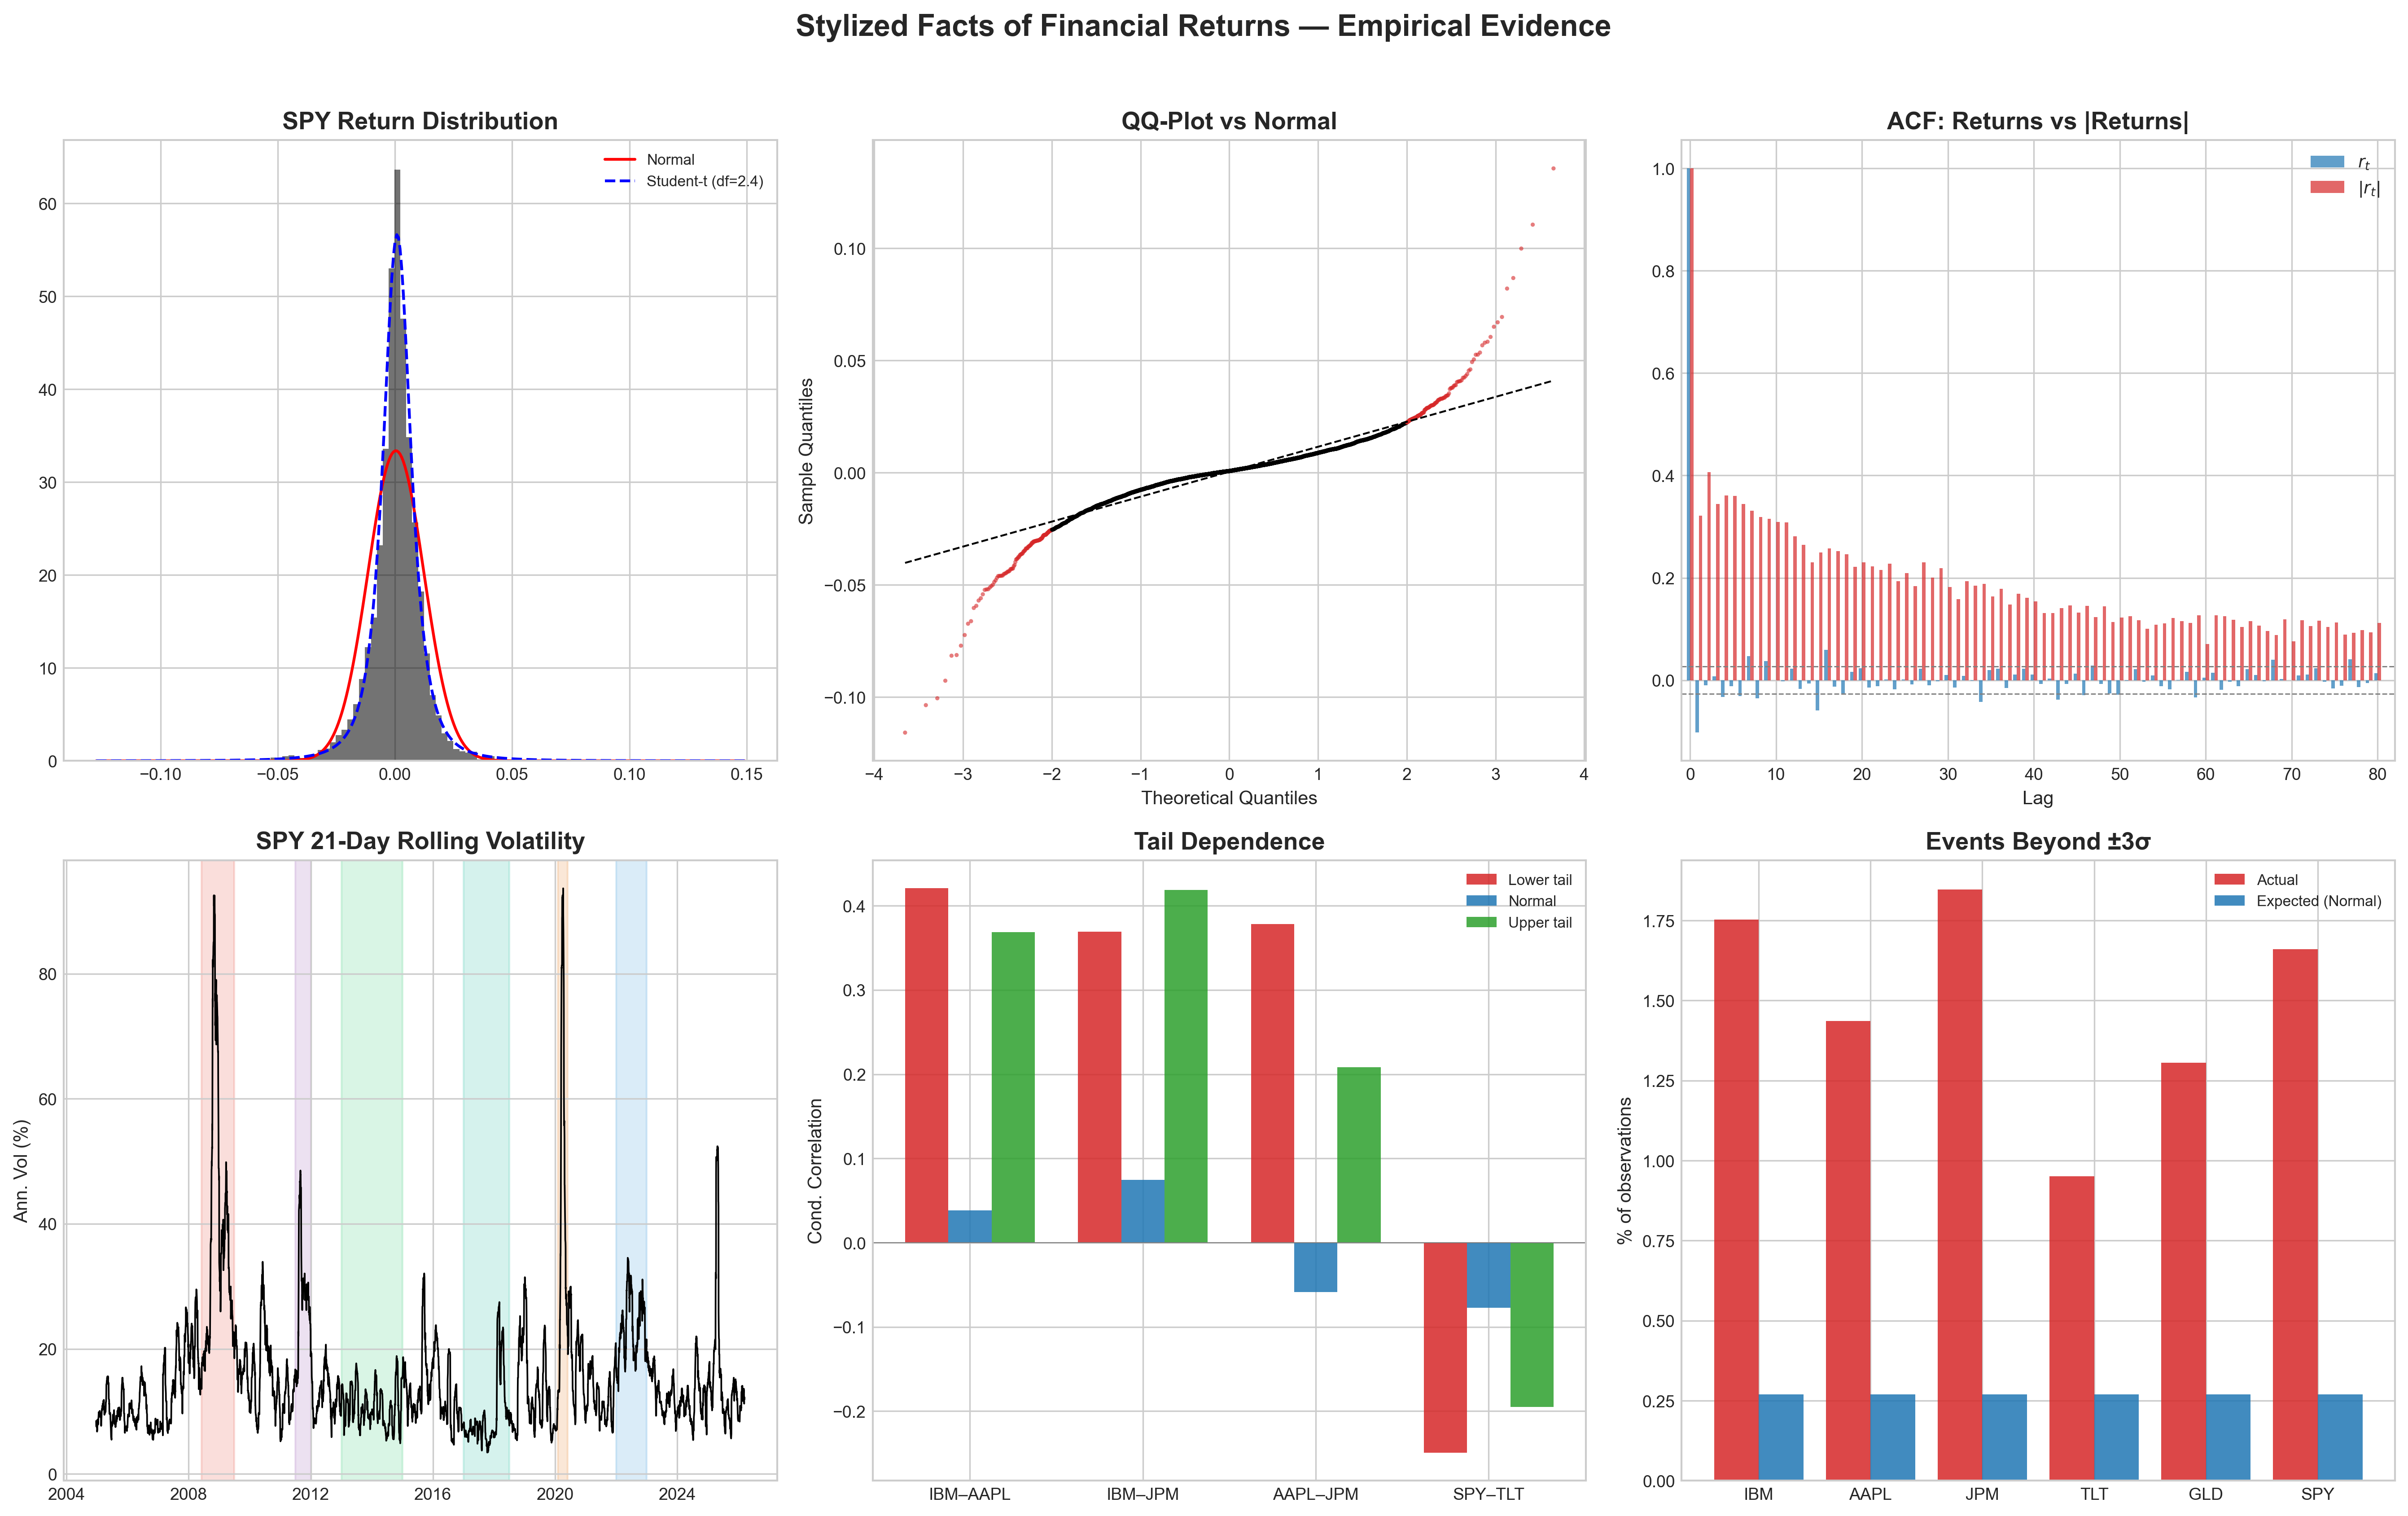
\includegraphics[width=\textwidth]{figures/summary_dashboard.png}
    \caption{Exploratory data analysis summary. \textbf{Top-left}: Return distribution histograms with fitted Gaussian overlay, showing the heavier tails of empirical returns. \textbf{Top-right}: QQ plots against the normal distribution, where departures from the diagonal indicate non-normality. \textbf{Bottom-left}: Rolling 60-day volatility showing pronounced clustering. \textbf{Bottom-right}: Correlation matrices by regime, revealing the asymmetric dependence structure that motivates vine copula modeling.}
    \label{fig:eda_summary}
\end{figure}


% ============================================================
\section{Deterministic Baseline Models}
\label{sec:deterministic}
% ============================================================

Before introducing stochastic volatility, we establish what deterministic models can and cannot achieve.
This section serves two purposes: (1) to benchmark point forecast accuracy across model classes, and (2) to demonstrate precisely \emph{why} point forecasts are insufficient for risk management---motivating the paradigm shift to probabilistic models.

% --- 3.1 ARIMA ---
\subsection{ARIMA --- Autoregressive Integrated Moving Average}
\label{sec:arima}

The ARIMA$(p,d,q)$ model for log-returns $r_t$ is given by:
\begin{equation}
\label{eq:arima}
r_t = c + \phi_1 r_{t-1} + \cdots + \phi_p r_{t-p} + \varepsilon_t + \theta_1 \varepsilon_{t-1} + \cdots + \theta_q \varepsilon_{t-q}
\end{equation}
where $\varepsilon_t \sim \mathcal{N}(0, \sigma^2)$ are i.i.d.\ innovations.
ARIMA combines three components:
\begin{itemize}[leftmargin=1.5em]
    \item \textbf{Autoregressive (AR):} The terms $\sum_{i=1}^{p} \phi_i r_{t-i}$ model the dependence of today's return on past returns, capturing short-term momentum or mean-reversion patterns. A positive $\phi_1$ indicates momentum (yesterday's positive return predicts a positive return today); a negative $\phi_1$ indicates mean-reversion.
    \item \textbf{Integrated (I):} The differencing order $d$ handles non-stationarity. Since log-returns are approximately stationary---confirmed by our Augmented Dickey--Fuller tests with $p < 0.001$ for all assets (Table~\ref{tab:adf})---we set $d = 0$ throughout.
    \item \textbf{Moving Average (MA):} The terms $\sum_{j=1}^{q} \theta_j \varepsilon_{t-j}$ model dependence on past forecast errors, allowing the model to correct for recent over- or under-predictions.
\end{itemize}

We use the auto-ARIMA algorithm \citep{hyndman2008} to select the optimal $(p, q)$ order by minimizing the Akaike Information Criterion (AIC), which balances goodness of fit against model complexity to guard against overfitting.
The selected orders are presented in Table~\ref{tab:arima_orders}.

\begin{table}[H]
\centering
\caption{Auto-ARIMA selected orders and AIC values. The low orders ($p + q \leq 4$) indicate minimal exploitable autocorrelation in log-returns.}
\label{tab:arima_orders}
\small
\begin{tabular}{@{}lrr@{}}
\toprule
\textbf{Asset} & \textbf{Order $(p,d,q)$} & \textbf{AIC} \\
\midrule
IBM  & $(1,0,0)$ & $-$24{,}241.0 \\
AAPL & $(0,0,1)$ & $-$21{,}124.3 \\
JPM  & $(1,0,3)$ & $-$20{,}084.3 \\
TLT  & $(0,0,3)$ & $-$28{,}455.4 \\
GLD  & $(0,0,0)$ & $-$26{,}364.5 \\
SPY  & $(0,0,1)$ & $-$25{,}850.0 \\
\bottomrule
\end{tabular}
\end{table}

\begin{table}[H]
\centering
\caption{Stationarity tests. ADF tests on prices fail to reject the unit root for 5 of 6 assets, confirming non-stationarity in levels. ADF tests on log-returns reject the unit root ($p < 0.001$) for all assets, confirming stationarity after differencing.}
\label{tab:adf}
\small
\begin{tabular}{@{}lrrrr@{}}
\toprule
\textbf{Asset} & \textbf{ADF (Price)} & \textbf{$p$-value} & \textbf{ADF (Return)} & \textbf{$p$-value} \\
\midrule
IBM  & $-$2.424 & 0.367 & $-$20.291 & $<$0.001 \\
AAPL & +2.156   & 1.000 & $-$15.242 & $<$0.001 \\
JPM  & $-$1.307 & 0.886 & $-$15.855 & $<$0.001 \\
TLT  & $-$3.512 & 0.038 & $-$21.092 & $<$0.001 \\
GLD  & $-$1.922 & 0.643 & $-$66.260 & $<$0.001 \\
SPY  & +0.497   & 0.997 & $-$16.116 & $<$0.001 \\
\bottomrule
\end{tabular}
\end{table}

The fundamental limitation of ARIMA is its assumption of \emph{homoscedastic} errors: $\varepsilon_t \sim \mathcal{N}(0, \sigma^2)$ with $\sigma^2$ constant over time.
This assumption is directly contradicted by the volatility clustering documented in Section~\ref{sec:volclustering}.
ARIMA's prediction intervals are computed as $\hat{r}_{t+1} \pm z_{\alpha/2} \cdot \hat{\sigma}$, where $\hat{\sigma}$ is estimated from the full training sample and \emph{remains fixed} regardless of current market conditions.
During calm periods, these intervals are too wide (wasting risk capital); during crises, they are too narrow (underestimating risk).

% --- 3.2 Random Forest and XGBoost ---
\subsection{Random Forest and XGBoost}
\label{sec:ml}

\textbf{Random Forest} \citep{breiman2001} constructs an ensemble of $B$ decision trees, each trained on a bootstrap sample of the data with a random subset of $\lfloor\sqrt{p}\rfloor$ features at each split.
The final prediction is the average across all trees:
\begin{equation}
\label{eq:rf}
\hat{r}_{t+1} = \frac{1}{B}\sum_{b=1}^{B} T_b(\mathbf{x}_t)
\end{equation}
where $T_b$ is the $b$-th decision tree and $\mathbf{x}_t$ is the feature vector at time $t$.
The averaging over decorrelated trees reduces variance relative to a single tree, while the bootstrap sampling and feature subsetting provide regularization against overfitting.

Our feature set includes: lagged returns at 1, 2, 3, 5, 10, and 20 days; rolling volatility at 5, 20, and 60 days; rolling skewness and kurtosis at 20 and 60 days; VIX level and daily change; and day-of-week indicators---25 engineered features in total.
Feature importance analysis reveals that VIX level (4.96\%) and VIX change (3.29\%) are the most predictive features, followed by short-term volatility measures.
Notably, lagged returns contribute modestly (each lag below 2.1\%), confirming the weak autocorrelation structure of daily equity returns.

\textbf{XGBoost} \citep{chen2016} differs from Random Forest in that trees are constructed \emph{sequentially}, with each tree fitting the residual errors of the ensemble built so far.
This gradient boosting procedure typically achieves lower bias than bagging (Random Forest) but is more susceptible to overfitting, which we control through $L_2$ regularization ($\lambda = 1$) and a conservative learning rate ($\eta = 0.01$).
The objective function at iteration $m$ is:
\begin{equation}
\label{eq:xgb}
\mathcal{L}^{(m)} = \sum_{i=1}^{T} \ell\bigl(r_i, \hat{r}_i^{(m-1)} + f_m(\mathbf{x}_i)\bigr) + \Omega(f_m)
\end{equation}
where $\ell$ is the squared-error loss, $f_m$ is the new tree, and $\Omega(f_m) = \gamma J + \frac{1}{2}\lambda \sum_{j=1}^{J} w_j^2$ penalizes tree complexity ($J$ leaves with weights $w_j$).

Both RF and XGBoost are \emph{deterministic} models: they output a single predicted value.
While the ensemble structure of RF can be used to construct pseudo-prediction intervals (using the distribution of individual tree predictions), these intervals are not calibrated---there is no theoretical guarantee that a ``95\% interval'' contains the true value 95\% of the time.
This is a fundamental limitation: ML models optimize for point prediction accuracy (RMSE), not for uncertainty quantification.

% --- 3.3 Results ---
\subsection{Results: Point Forecasts Are Nearly Futile}
\label{sec:det_results}

All models are evaluated using walk-forward (expanding window) cross-validation on the period 2022--2025, with one-step-ahead daily forecasts.
Table~\ref{tab:rmse} presents point forecast accuracy.

\begin{table}[H]
\centering
\caption{Point forecast metrics across models and assets (walk-forward evaluation, 2022--2025). RMSE is root mean squared error; Dir.\ Acc.\ is directional accuracy (percentage of days where the predicted sign matches the realized sign). The Random Walk baseline predicts zero return.}
\label{tab:rmse}
\small
\begin{tabular}{@{}llrrrr@{}}
\toprule
\textbf{Model} & \textbf{Asset} & \textbf{RMSE} & \textbf{MAE} & \textbf{Dir.\ Acc.\ (\%)} \\
\midrule
Random Walk   & SPY & 0.01117 & 0.00785 & ---   \\
ARIMA         & SPY & 0.01120 & 0.00792 & 50.5  \\
Random Forest & SPY & 0.01116 & 0.00793 & 52.9  \\
XGBoost       & SPY & 0.01126 & 0.00803 & 49.7  \\
\midrule
Random Walk   & IBM & ---     & ---     & ---   \\
ARIMA         & IBM & 0.01618 & 0.01083 & 50.9  \\
Random Forest & IBM & 0.01622 & 0.01088 & 53.1  \\
XGBoost       & IBM & 0.01640 & 0.01100 & 49.3  \\
\bottomrule
\end{tabular}
\end{table}

Table~\ref{tab:rmse} reveals a striking result: no model meaningfully outperforms the random walk baseline.
Random Forest achieves an RMSE of 0.01116 on SPY, compared to the random walk's 0.01117---a difference that vanishes at the fifth decimal place.
This is not a failure of implementation; it is a fundamental property of daily equity returns.
The efficient market hypothesis \citep{fama1970} predicts that returns are approximately unpredictable on short horizons, and our results confirm this empirically across multiple model classes.

Directional accuracy tells a similar story: the best model (Random Forest at 53.1\% for IBM) is barely better than a fair coin.
The practical implication is clear: allocating computational resources to improve point forecasts of daily returns yields negligible benefit.
The question is not whether we can predict the price, but whether we can characterize the \emph{distribution} of possible outcomes.

% --- 3.4 Prediction Interval Failure ---
\subsection{Prediction Interval Failure --- The Motivation for Probabilistic Models}
\label{sec:pi_failure}

The most consequential failure of deterministic models is not in their point forecasts but in their prediction intervals.
ARIMA produces 95\% prediction intervals using $\hat{r}_{t+1} \pm 1.96\hat{\sigma}$, where $\hat{\sigma}$ is estimated once from the training window and held constant.
Table~\ref{tab:coverage} presents empirical coverage by market regime.

\begin{table}[H]
\centering
\caption{ARIMA 95\% prediction interval coverage by market regime. Crisis periods are defined as days when the 20-day realized volatility of SPY exceeds its 80th percentile. The target coverage is 95\%.}
\label{tab:coverage}
\small
\begin{tabular}{@{}lrrrrr@{}}
\toprule
\textbf{Asset} & \textbf{Overall (\%)} & \textbf{Crisis (\%)} & \textbf{Calm (\%)} & \textbf{Avg PI Width} \\
\midrule
IBM  & 95.1 & 95.2 & 95.0 & 0.0568 \\
AAPL & 96.6 & 94.0 & 97.4 & 0.0808 \\
JPM  & 97.8 & 96.8 & 98.1 & 0.0898 \\
SPY  & 96.1 & 88.4 & 98.5 & 0.0473 \\
\bottomrule
\end{tabular}
\end{table}

SPY reveals the critical failure: ARIMA's 95\% prediction intervals achieve only 88.4\% empirical coverage during crisis periods---seven percentage points below the stated confidence level.
This means that on approximately one in nine crisis days, the actual loss exceeds the model's stated ``worst case.''
Meanwhile, during calm markets, coverage is 98.5\%---three percentage points above target---meaning the intervals are unnecessarily wide and tie up more risk capital than needed.

\begin{figure}[H]
    \centering
    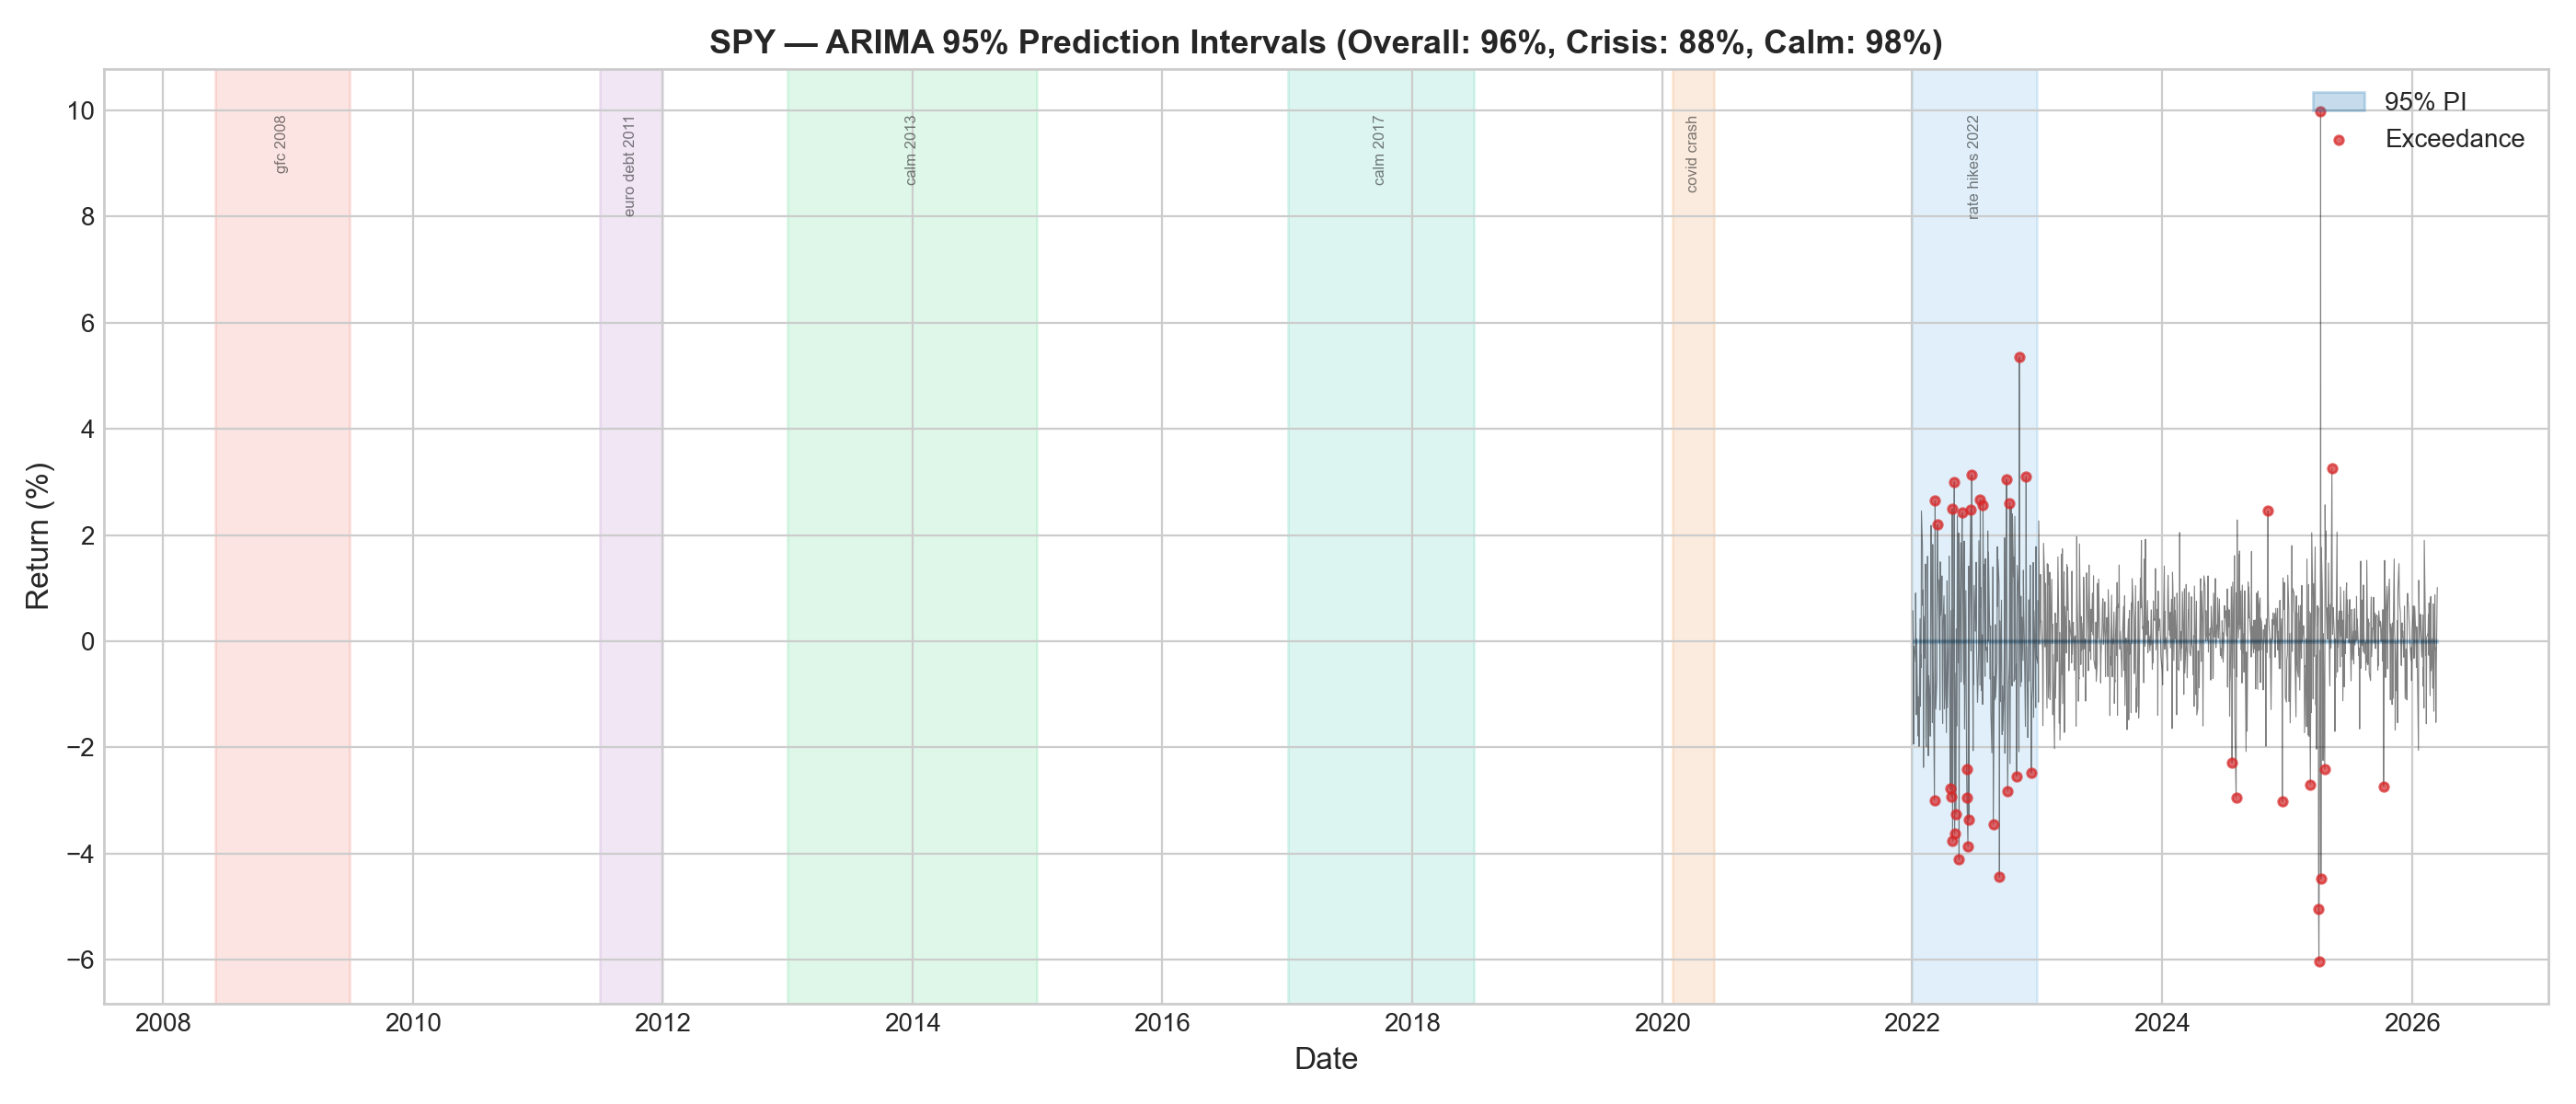
\includegraphics[width=\textwidth]{figures/prediction_intervals_spy.png}
    \caption{ARIMA prediction intervals on SPY daily returns. The shaded band shows the 95\% interval; red markers indicate exceedances (days when the realized return falls outside the interval). Exceedances cluster during high-volatility regimes (2022 inflation shock, 2023 banking stress), demonstrating that ARIMA's constant-width intervals cannot adapt to time-varying volatility.}
    \label{fig:arima_pi}
\end{figure}

Exceedance clustering analysis (Table~\ref{tab:exceedance}) provides further evidence.
For ARIMA on SPY at the 99\% level, the clustering ratio is 10.64$\times$: if the model's VaR was violated today, it is 10.64 times more likely to be violated again tomorrow than on a random day.
This clustering means that ARIMA's failures concentrate into multi-day streaks---precisely the scenario that produces the largest cumulative losses and poses the greatest threat to institutional solvency.

\begin{table}[H]
\centering
\caption{Exceedance clustering analysis for ARIMA on SPY (99\% VaR, 1{,}053 test days). $P(\text{exceed})$ is the unconditional exceedance probability; $P(\text{exceed}|\text{prev})$ is the probability of exceedance given that the previous day also exceeded. The clustering ratio reveals severe serial dependence in VaR violations.}
\label{tab:exceedance}
\small
\begin{tabular}{@{}lrrrrr@{}}
\toprule
$P(\text{exceed})$ & $P(\text{exceed}|\text{prev})$ & \textbf{Clustering Ratio} & \textbf{Longest Streak} & \textbf{Exceedances} \\
\midrule
3.89\% & 14.63\% & 10.64$\times$ & 3 days & 41 / 1{,}053 \\
\bottomrule
\end{tabular}
\end{table}

\subsubsection{The Deterministic--Probabilistic Divide}
\label{sec:det_vs_prob}

The failures documented above are not accidental; they are \emph{structural}.
Deterministic models share a fundamental architectural limitation: they produce a single predicted value surrounded by a fixed-width confidence band.
This design implicitly assumes that the uncertainty around a prediction is constant---an assumption directly contradicted by volatility clustering.

Consider the two desiderata of a risk model:
\begin{enumerate}[leftmargin=1.5em]
    \item \textbf{Correct average coverage:} Over a long period, the fraction of exceedances should match the target rate (e.g., 1\% for VaR$_{99}$). ARIMA achieves this for some assets (Kupiec $p = 0.193$ for SPY at 99\%).
    \item \textbf{Independent exceedances:} Violations should not cluster---each day's exceedance should be independent of the previous day's. ARIMA fails this (Christoffersen $p = 0.023$ for SPY at 99\%).
\end{enumerate}

A model can satisfy the first criterion while catastrophically failing the second---and the second is far more dangerous in practice.
A risk system with 1\% average exceedance rate but severe clustering produces multi-day loss streaks that are far more damaging than evenly-distributed violations.
An institution can survive one day of unexpected losses; a week of consecutive VaR breaches triggers margin calls, forced liquidations, and regulatory action.

These results motivate a fundamental shift in approach.
Rather than asking ``What will the return be?'' (a question whose answer is approximately ``we cannot know,'' per the efficient market evidence above), we ask ``What is the full distribution of possible returns, and how does it change with market conditions?''
This is the probabilistic paradigm: replacing point forecasts with \emph{distributional} forecasts, and replacing constant uncertainty bands with models whose uncertainty estimates \emph{adapt to the current volatility regime}.

\begin{figure}[H]
    \centering
    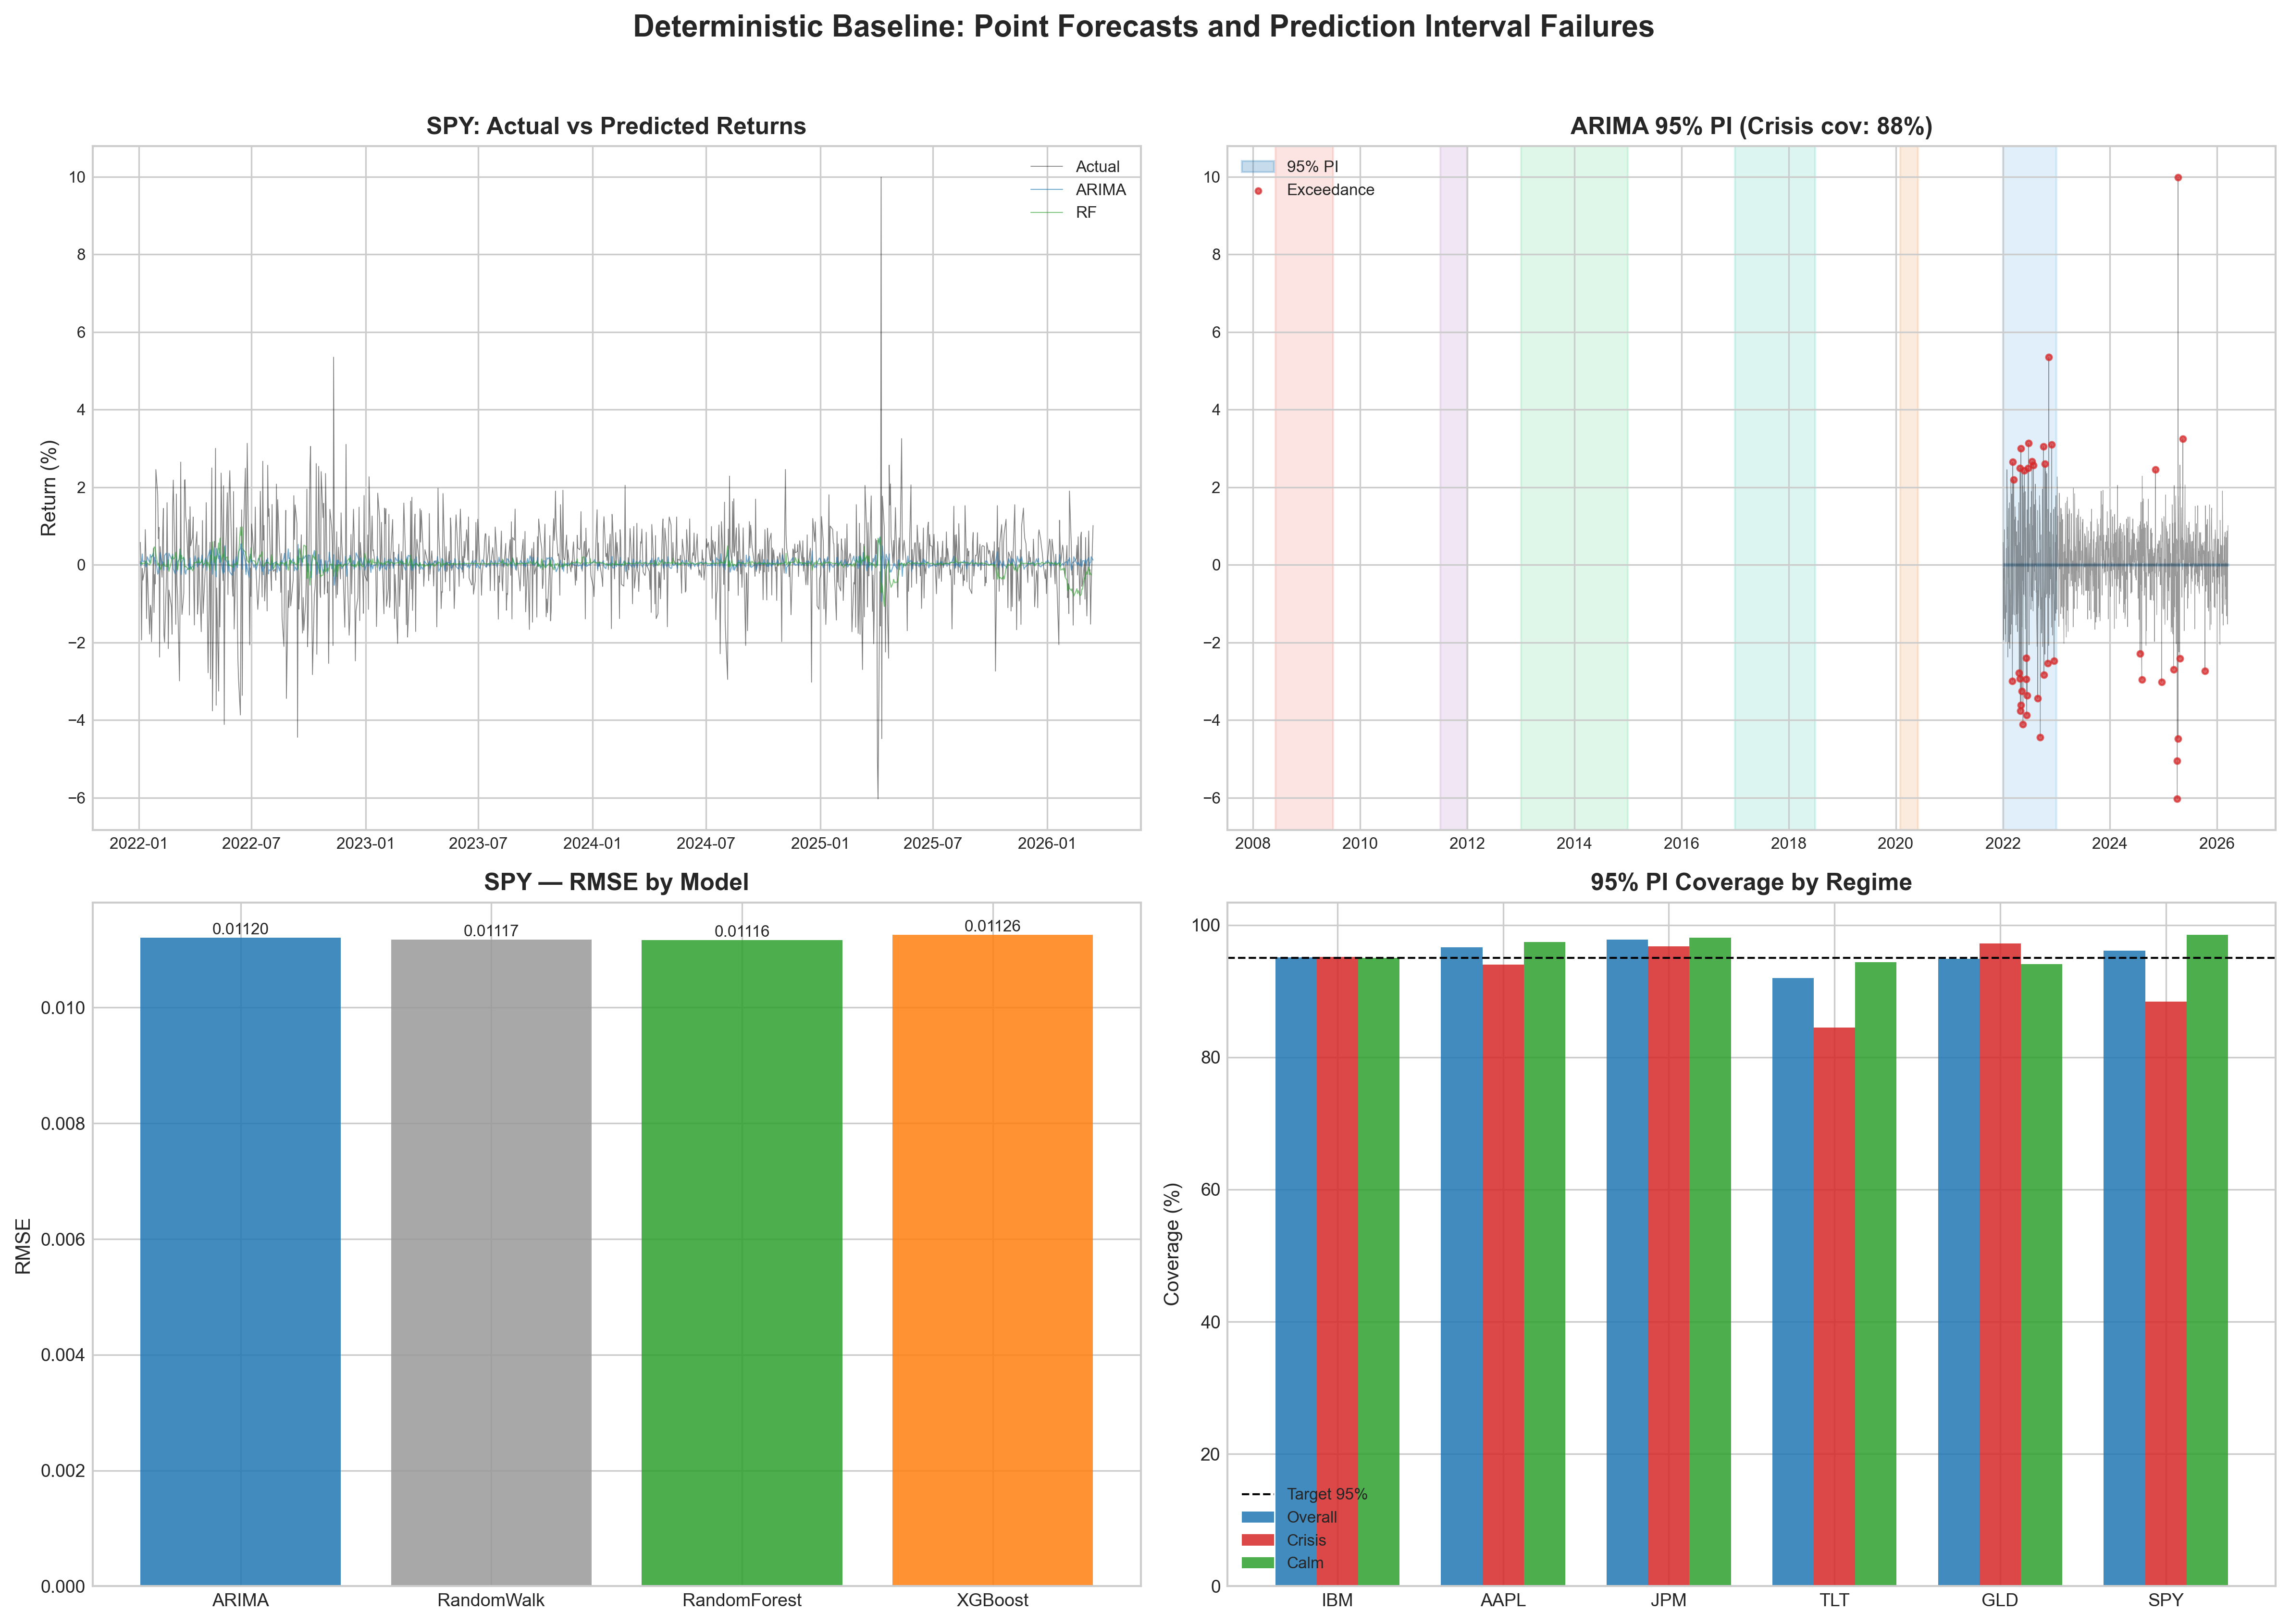
\includegraphics[width=\textwidth]{figures/baseline_summary.png}
    \caption{Baseline model comparison summary. \textbf{Left}: RMSE across all models and assets, showing near-identical performance. \textbf{Right}: Feature importance from Random Forest, with VIX level and short-term volatility features dominating---the model learns that volatility is predictable even when returns are not.}
    \label{fig:baseline_summary}
\end{figure}


% ============================================================
\section{Stochastic Volatility Framework}
\label{sec:stochvol}
% ============================================================

% --- 4.1 GBM ---
\subsection{Geometric Brownian Motion}
\label{sec:gbm}

The simplest continuous-time model for asset prices is Geometric Brownian Motion, first applied to option pricing by \citet{black1973} and \citet{merton1973}:
\begin{equation}
\label{eq:gbm}
dS_t = \mu S_t \, dt + \sigma S_t \, dW_t
\end{equation}
where:
\begin{itemize}[leftmargin=1.5em]
    \item $S_t$ is the asset price at time $t$.
    \item $\mu$ is the drift rate (annualized expected return), representing the risk premium investors demand for holding the asset. For our assets, calibrated values range from $\mu = 0.032$ (TLT) to $\mu = 0.269$ (AAPL).
    \item $\sigma$ is the volatility (annualized standard deviation of log-returns), assumed \textbf{constant} over time. This single assumption is both the model's strength---it yields the closed-form Black--Scholes option pricing formula---and its fundamental weakness, since real volatility is demonstrably time-varying (Section~\ref{sec:volclustering}).
    \item $dW_t$ is the increment of a standard Brownian motion, a random shock drawn from $\mathcal{N}(0, dt)$. It represents the unpredictable component of returns.
\end{itemize}

The exact solution is:
\begin{equation}
\label{eq:gbm_solution}
S_T = S_0 \exp\!\left[\left(\mu - \tfrac{\sigma^2}{2}\right)T + \sigma W_T\right]
\end{equation}
yielding log-normal terminal prices.
This closed-form solution serves two purposes in our framework: (1) as the simplest baseline model against which we measure model risk, and (2) as an analytical control variate for variance reduction (Section~\ref{sec:vr}), where the known analytical moments of GBM reduce the variance of Heston Monte Carlo estimates by exploiting the high correlation ($\rho = 0.69$) between GBM and Heston terminal values.

% --- 4.2 Heston ---
\subsection{Heston Stochastic Volatility Model}
\label{sec:heston}

\citet{heston1993} introduced stochastic volatility by coupling the price process to a mean-reverting variance process:
\begin{align}
\label{eq:heston}
dS_t &= \mu S_t \, dt + \sqrt{v_t} \, S_t \, dW_t^{(1)} \\
dv_t &= \kappa(\theta - v_t) \, dt + \sigma_v \sqrt{v_t} \, dW_t^{(2)} \label{eq:heston_var}
\end{align}
with $\Corr(dW_t^{(1)}, dW_t^{(2)}) = \rho$.
The five parameters govern distinct financial phenomena:

\textbf{$\kappa$ (mean-reversion speed).}
Controls how rapidly variance returns to its long-run level after a shock.
The half-life of a variance perturbation is $\ln(2)/\kappa$---with our calibrated $\kappa = 0.608$ for SPY, a volatility spike dissipates to half its excess within approximately 14 months.
Higher $\kappa$ means shorter-lived volatility regimes; lower $\kappa$ produces persistent volatility clustering similar to what we observe empirically.

\textbf{$\theta$ (long-run variance).}
The equilibrium level to which variance reverts.
Our calibrated $\theta = 0.1056$ for SPY corresponds to a long-run annualized volatility of $\sqrt{0.1056} = 32.5\%$.
The mean-reverting drift $\kappa(\theta - v_t)$ acts as a spring: when current variance $v_t$ exceeds $\theta$, the drift pulls it down; when $v_t < \theta$, the drift pushes it up.

\textbf{$\sigma_v$ (volatility of volatility).}
Determines how erratically the variance process evolves around its mean.
Our calibrated $\sigma_v = 0.810$ for SPY indicates substantial variance variability.
Higher $\sigma_v$ produces more dramatic variance swings, which translates directly into heavier tails in the return distribution---the mechanism by which Heston generates excess kurtosis that matches the empirical values in Table~\ref{tab:summary}.

\textbf{$\rho$ (leverage correlation).}
The correlation between the Brownian motions driving price and variance.
Empirically negative for equities: our calibrated $\rho = -0.287$ for SPY.
When prices fall ($dW^{(1)} < 0$), variance tends to rise ($dW^{(2)} > 0$ through the correlation).
This is the \emph{leverage effect} first documented by \citet{black1976}---named because falling stock prices increase a firm's financial leverage, increasing perceived risk and thus volatility.
Negative $\rho$ produces the negative skewness observed in equity return distributions: crash scenarios are amplified (falling price + rising volatility) while rallies are dampened.

\textbf{$v_0$ (initial variance).}
The starting value of the variance process.
We estimate $v_0$ from recent realized volatility: $v_0 = \hat{\sigma}_{20d}^2$.
For SPY, $v_0 = 0.01349$.

The \textbf{Feller condition} $2\kappa\theta > \sigma_v^2$ ensures the variance process never reaches zero.
With our calibrated parameters, $2 \times 0.608 \times 0.1056 = 0.128 < 0.810^2 = 0.656$, so the Feller condition is \emph{violated}---a common occurrence with empirically calibrated parameters.
The standard Euler--Maruyama discretization can then produce negative variances.
We resolve this by implementing the QE (Quadratic-Exponential) scheme of \citet{andersen2008}, which eliminates negative-variance artifacts through a switching rule between quadratic and exponential moment-matching regimes based on the ratio $\psi = s^2/m^2$ (where $m$ and $s^2$ are the conditional mean and variance of $v_{t+\Delta t}$).

\begin{table}[H]
\centering
\caption{Calibrated parameters via maximum likelihood estimation (MLE) on historical returns. The Feller condition ($2\kappa\theta > \sigma_v^2$) is violated for all assets, necessitating the QE discretization scheme.}
\label{tab:calibration}
\small
\begin{tabular}{@{}llrrrrrr@{}}
\toprule
\textbf{Asset} & \textbf{Model} & $\kappa$ & $\theta$ & $\sigma_v$ & $\rho$ & $v_0$ & \textbf{Feller?} \\
\midrule
SPY & Heston        & 0.608 & 0.1056  & 0.810 & $-$0.287 & 0.0135 & No \\
SPY & Rough Heston  & 0.485 & 0.00358 & 0.530 & $-$0.198 & 0.0451 & No \\
IBM & Heston        & 0.500 & 0.0541  & 0.161 & $-$0.087 & 0.1234 & No \\
JPM & Heston        & 0.500 & ---     & ---   & ---      & ---    & No \\
\bottomrule
\end{tabular}
\end{table}

% --- 4.3 Rough Heston ---
\subsection{Rough Heston}
\label{sec:rough_heston}

\citet{gatheral2018} made a striking empirical discovery: the log-volatility of asset prices behaves as a \emph{fractional} Brownian motion with Hurst exponent $H \approx 0.1$---far below the $H = 0.5$ of standard Brownian motion.
The Rough Heston model replaces Heston's Markovian variance dynamics with a Volterra integral equation:
\begin{equation}
\label{eq:rough_heston}
v_t = v_0 + \frac{1}{\Gamma(H + \tfrac{1}{2})} \int_0^t (t-s)^{H-\frac{1}{2}} \left[\kappa(\theta - v_s)\,ds + \sigma_v \sqrt{v_s}\,dW_s^{(2)}\right]
\end{equation}

\textbf{$H$ (Hurst exponent).}
Controls the roughness and memory of the volatility process.
At $H = 0.5$, the fractional kernel reduces to a delta function and Rough Heston becomes exactly classical Heston---we verify this numerically.
At our calibrated $H = 0.13$ for SPY, the kernel $(t-s)^{-0.37}$ weights recent history heavily (the function diverges as $s \to t$) while retaining influence from the distant past (the function decays slowly as $s \to 0$).
This produces two simultaneous effects:
\begin{enumerate}[leftmargin=1.5em]
    \item Volatility paths are \emph{rougher} at fine time scales---more jagged, higher-frequency variation than classical Heston.
    \item Volatility has \emph{longer memory} at coarse scales---the ACF decays as a power law $\rho_k \sim k^{2H-1}$ rather than exponentially, better matching the empirical ACF decay observed in Section~\ref{sec:volclustering}.
\end{enumerate}
Our calibrated $H = 0.13$ confirms the empirical finding of \citet{gatheral2018} and is consistent with estimates from implied volatility surface dynamics across global equity markets.

\textbf{Markovian approximation.}
The integral form makes the process non-Markovian: the variance at time $t$ depends on the entire history $\{v_s : 0 \leq s \leq t\}$, not just the current state.
Direct simulation requires $O(N^2)$ operations per path (each of $N$ time steps integrates over all previous steps), making large-scale Monte Carlo prohibitively expensive.

We resolve this through spectral approximation: the fractional kernel is decomposed as a weighted sum of exponentials,
\begin{equation}
\label{eq:kernel_approx}
\frac{t^{H-1/2}}{\Gamma(H+\tfrac{1}{2})} \approx \sum_{i=1}^{N_f} w_i \, e^{-\lambda_i t}
\end{equation}
where the rates $\lambda_i$ are distributed log-uniformly on $[\lambda_{\min}, \lambda_{\max}]$ and the weights $w_i$ are computed by least-squares fitting.
Each exponential term is Markovian (updatable in $O(1)$ per step), transforming the problem into a system of $N_f$ coupled SDEs.
With $N_f = 8$ factors, the relative $L^2$ kernel error is below 5\%, and risk metrics converge to within 0.01\% of higher-factor solutions.

% --- 4.4 Model Hierarchy ---
\subsection{Model Hierarchy and the Measurement of Model Risk}
\label{sec:hierarchy}

The three models form a nested hierarchy of increasing realism:
\begin{itemize}[leftmargin=1.5em]
    \item \textbf{GBM:} Constant volatility $\to$ captures none of the stylized facts documented in Section~\ref{sec:eda}. Serves as the null model.
    \item \textbf{Heston:} Stochastic volatility $\to$ captures fat tails (via $\sigma_v$), negative skewness (via $\rho < 0$), and short-term volatility clustering (via $\kappa$).
    \item \textbf{Rough Heston:} Rough stochastic volatility $\to$ additionally captures long-memory volatility dynamics (via $H < 0.5$) and finer tail structure.
\end{itemize}

The differences between their risk estimates constitute our measure of \emph{model risk}.
If all three models agreed, model choice would not matter.
The fact that they disagree by up to 31\% on ES$_{99}$ (Section~\ref{sec:risk_comparison}) demonstrates that model risk is material and comparable in magnitude to the market risk that the models attempt to measure.

\begin{figure}[H]
    \centering
    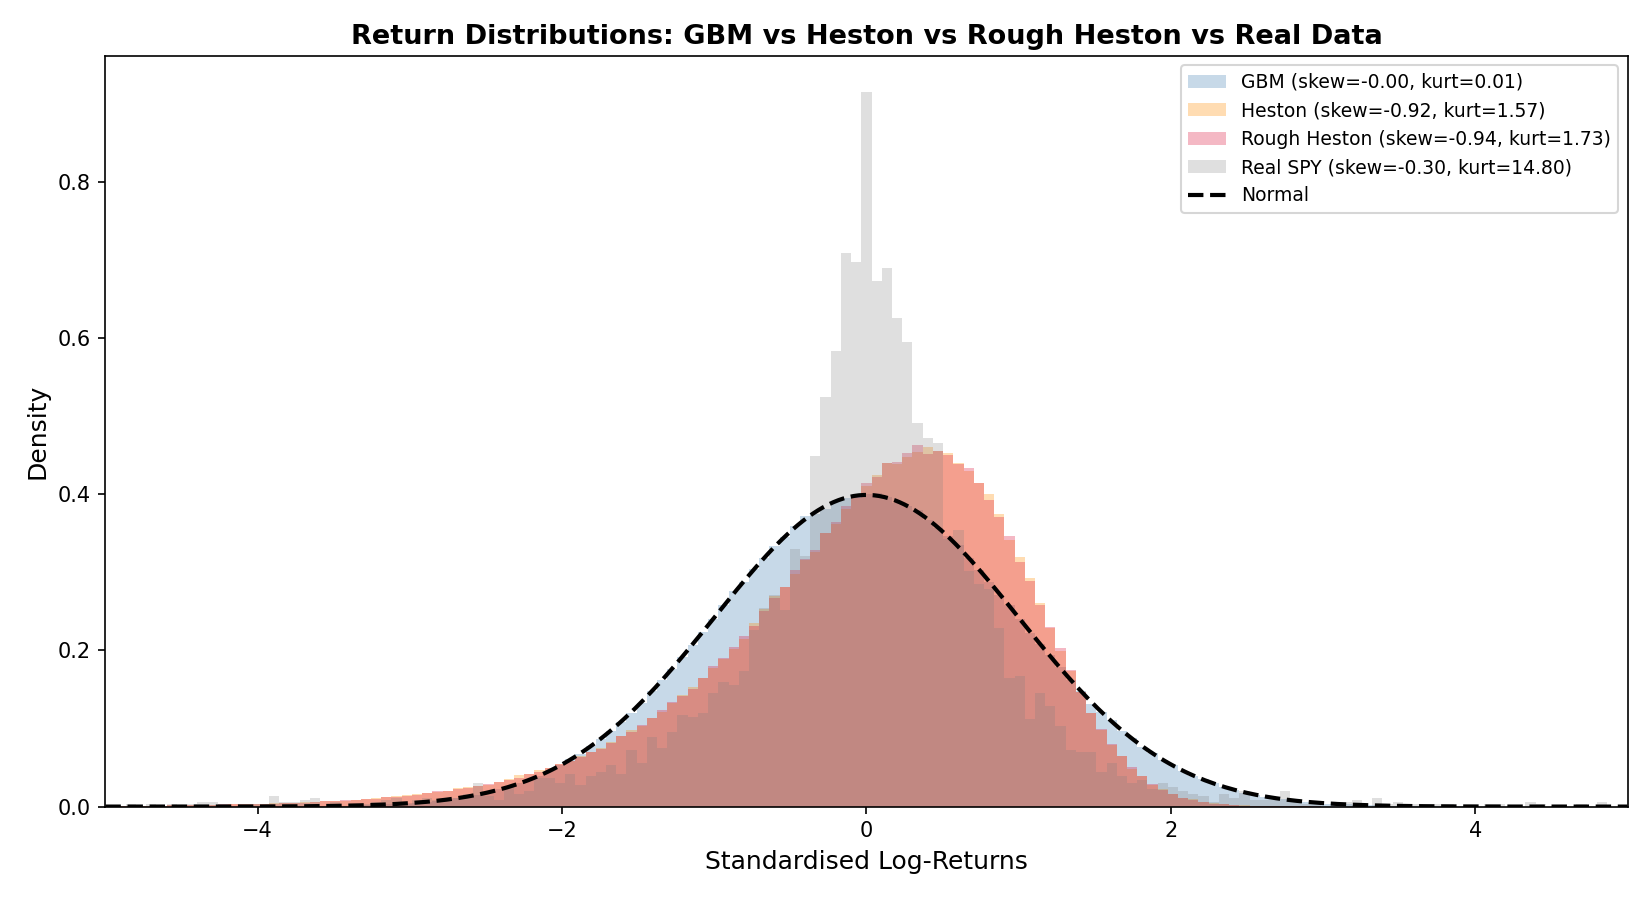
\includegraphics[width=\textwidth]{figures/three_model_distributions.png}
    \caption{Simulated return distributions under the three volatility models (100{,}000 paths each, SPY parameters). GBM produces symmetric, thin-tailed returns. Heston generates negative skewness and heavier tails. Rough Heston produces the heaviest tails and most pronounced negative skewness. The differences in the left tail directly translate to differences in VaR and ES estimates.}
    \label{fig:three_models}
\end{figure}


% ============================================================
\section{Multi-Asset Dependence with Vine Copulas}
\label{sec:copula}
% ============================================================

% --- 5.1 Copulas ---
\subsection{Copulas and Sklar's Theorem}
\label{sec:sklars}

Portfolio risk depends not only on individual asset distributions but on their joint behavior---particularly during market stress.
\citet{sklar1959} established the foundational decomposition theorem:

\begin{definition}[Sklar's Theorem]
Any multivariate distribution function $F$ with marginals $F_1, \ldots, F_d$ can be written~as:
\begin{equation}
\label{eq:sklar}
F(x_1, \ldots, x_d) = C\bigl(F_1(x_1), \ldots, F_d(x_d)\bigr)
\end{equation}
where $C : [0,1]^d \to [0,1]$ is a copula function that captures the entire dependence structure, independent of the marginal distributions.
\end{definition}

This decomposition is powerful because it allows us to model marginals and dependence \emph{separately}.
We use stochastic volatility models (Section~\ref{sec:stochvol}) for realistic marginal distributions (fat tails, skewness) and copulas for realistic dependence (tail dependence, asymmetry).
A Gaussian copula---implicit in any analysis using only Pearson correlation---forces symmetric dependence with zero tail dependence: the probability that two assets simultaneously experience extreme losses approaches zero in the Gaussian copula, regardless of their correlation.
Our vine copula allows each pair of assets to exhibit different tail dependence in crashes versus rallies \citep{nelsen2006}.

% --- 5.2 Vine Copula ---
\subsection{Vine Copula Structure}
\label{sec:vine}

For $d > 2$ assets, specifying a full multivariate copula directly is infeasible.
Vine copulas \citep{aas2009} decompose the $d$-dimensional dependence into a cascade of bivariate copulas organized in a tree structure.
We employ a C-vine (canonical vine) with SPY as the root variable, reflecting its role as the dominant driver of equity market risk.

Each edge in the vine is fitted with a bivariate Student-$t$ copula, which captures both upper and lower tail dependence symmetrically through the degrees-of-freedom parameter.
The lower tail dependence coefficient for a bivariate Student-$t$ copula with correlation $\rho$ and $\nu$ degrees of freedom is:
\begin{equation}
\label{eq:lambda_t}
\lambda_L = \lambda_U = 2\,t_{\nu+1}\!\left(-\sqrt{\frac{(\nu+1)(1-\rho)}{1+\rho}}\right)
\end{equation}
where $t_{\nu+1}$ is the CDF of the Student-$t$ distribution with $\nu + 1$ degrees of freedom.
As $\nu \to \infty$, $\lambda_L \to 0$ (recovering the Gaussian copula's zero tail dependence); smaller $\nu$ produces stronger tail dependence.

Table~\ref{tab:vine} presents the fitted vine copula structure for our six-asset portfolio.

\begin{table}[H]
\centering
\caption{Vine copula structure (Tree 1, unconditional pairs). All pairs are fitted with Student-$t$ copulas except IBM--AAPL (Frank copula, zero tail dependence). The SPY--JPM pair exhibits the strongest tail dependence ($\lambda = 0.407$).}
\label{tab:vine}
\small
\begin{tabular}{@{}llrrrr@{}}
\toprule
\textbf{Edge} & \textbf{Family} & \textbf{$\rho$} & \textbf{$\nu$} & $\lambda_L$ & $\lambda_U$ \\
\midrule
TLT--JPM  & Student-$t$ & 0.184 & 5.89 & 0.066 & 0.066 \\
SPY--JPM  & Student-$t$ & 0.657 & 3.12 & 0.407 & 0.407 \\
SPY--IBM  & Student-$t$ & $-$0.055 & 5.82 & 0.029 & 0.029 \\
IBM--AAPL & Frank       & $-$0.294 & ---  & 0     & 0     \\
\bottomrule
\end{tabular}
\end{table}

% --- 5.3 Results ---
\subsection{Copula Impact on Portfolio Risk}
\label{sec:copula_results}

Table~\ref{tab:copula_risk} presents portfolio risk metrics under four dependence assumptions, from independence to perfect comonotonicity.
All use the same Heston-calibrated marginals with equal portfolio weights.

\begin{table}[H]
\centering
\caption{Portfolio risk metrics under different dependence structures (equal-weighted six-asset portfolio, Heston marginals). Independent: assets are uncorrelated. Gaussian: linear correlation only. Vine: Student-$t$ vine copula with tail dependence. Comonotonic: perfect positive dependence (upper bound).}
\label{tab:copula_risk}
\small
\begin{tabular}{@{}lrrrrrr@{}}
\toprule
\textbf{Dependence} & \textbf{VaR$_{95}$} & \textbf{VaR$_{99}$} & \textbf{ES$_{95}$} & \textbf{ES$_{99}$} & $P(\text{loss}>5\%)$ \\
\midrule
Independent   & 0.94\% & 1.68\% & 1.48\% & 2.62\% & 0.047\% \\
Gaussian      & 1.28\% & 2.44\% & 2.09\% & 3.78\% & 0.135\% \\
Vine Copula   & 1.24\% & 2.55\% & 2.21\% & 4.34\% & 0.192\% \\
Comonotonic   & 2.08\% & 4.16\% & 3.55\% & 6.64\% & 0.624\% \\
\bottomrule
\end{tabular}
\end{table}

The vine copula produces ES$_{99}$ of 4.34\%, compared to the Gaussian copula's 3.78\%---a 15\% increase arising purely from modeling asymmetric tail dependence.
The Gaussian copula underestimates tail risk because it cannot capture the phenomenon documented in Section~\ref{sec:taildep}: correlations increase during crises.
The vine copula, through its Student-$t$ pair copulas with low degrees of freedom (Table~\ref{tab:vine}), assigns positive probability to simultaneous extreme losses---the joint tail events that drive portfolio risk during market stress.

The probability of losses exceeding 5\% is 4.1$\times$ higher under the vine copula (0.192\%) than under independence (0.047\%), reflecting the loss of diversification during tail events.
This ``diversification failure'' is invisible to any risk framework based solely on linear correlation.

\textbf{Euler risk allocation} decomposes total portfolio ES into per-asset contributions:

\begin{table}[H]
\centering
\caption{Euler decomposition of vine copula ES$_{99}$. The ratio column shows risk contribution relative to portfolio weight. JPM contributes 2.3$\times$ its weight; TLT contributes negatively (genuine crash hedge).}
\label{tab:euler}
\small
\begin{tabular}{@{}lrrrr@{}}
\toprule
\textbf{Asset} & \textbf{Weight} & \textbf{ES Contribution} & \textbf{\% of ES} & \textbf{Ratio} \\
\midrule
IBM  & 16.7\% & 0.79\% & 18.2\% & 1.09$\times$ \\
AAPL & 16.7\% & 0.98\% & 22.6\% & 1.35$\times$ \\
JPM  & 16.7\% & 1.65\% & 38.1\% & 2.28$\times$ \\
TLT  & 16.7\% & $-$0.10\% & $-$2.3\% & hedge \\
GLD  & 16.7\% & 0.10\% & 2.3\%  & 0.14$\times$ \\
SPY  & 16.7\% & 0.92\% & 21.2\% & 1.27$\times$ \\
\bottomrule
\end{tabular}
\end{table}

JPM contributes 38.1\% of tail risk from only 16.7\% of portfolio weight---its risk contribution is 2.28$\times$ its allocation.
This asymmetry is driven by JPM's extreme kurtosis (18.23, Table~\ref{tab:summary}) and strong tail dependence with SPY ($\lambda = 0.407$).
TLT contributes \emph{negatively} ($-$2.3\%): during equity crashes, bond prices tend to rise, providing genuine hedging that reduces portfolio tail risk.
This information is invisible to a manager who examines only portfolio weights and correlations.

\begin{figure}[H]
    \centering
    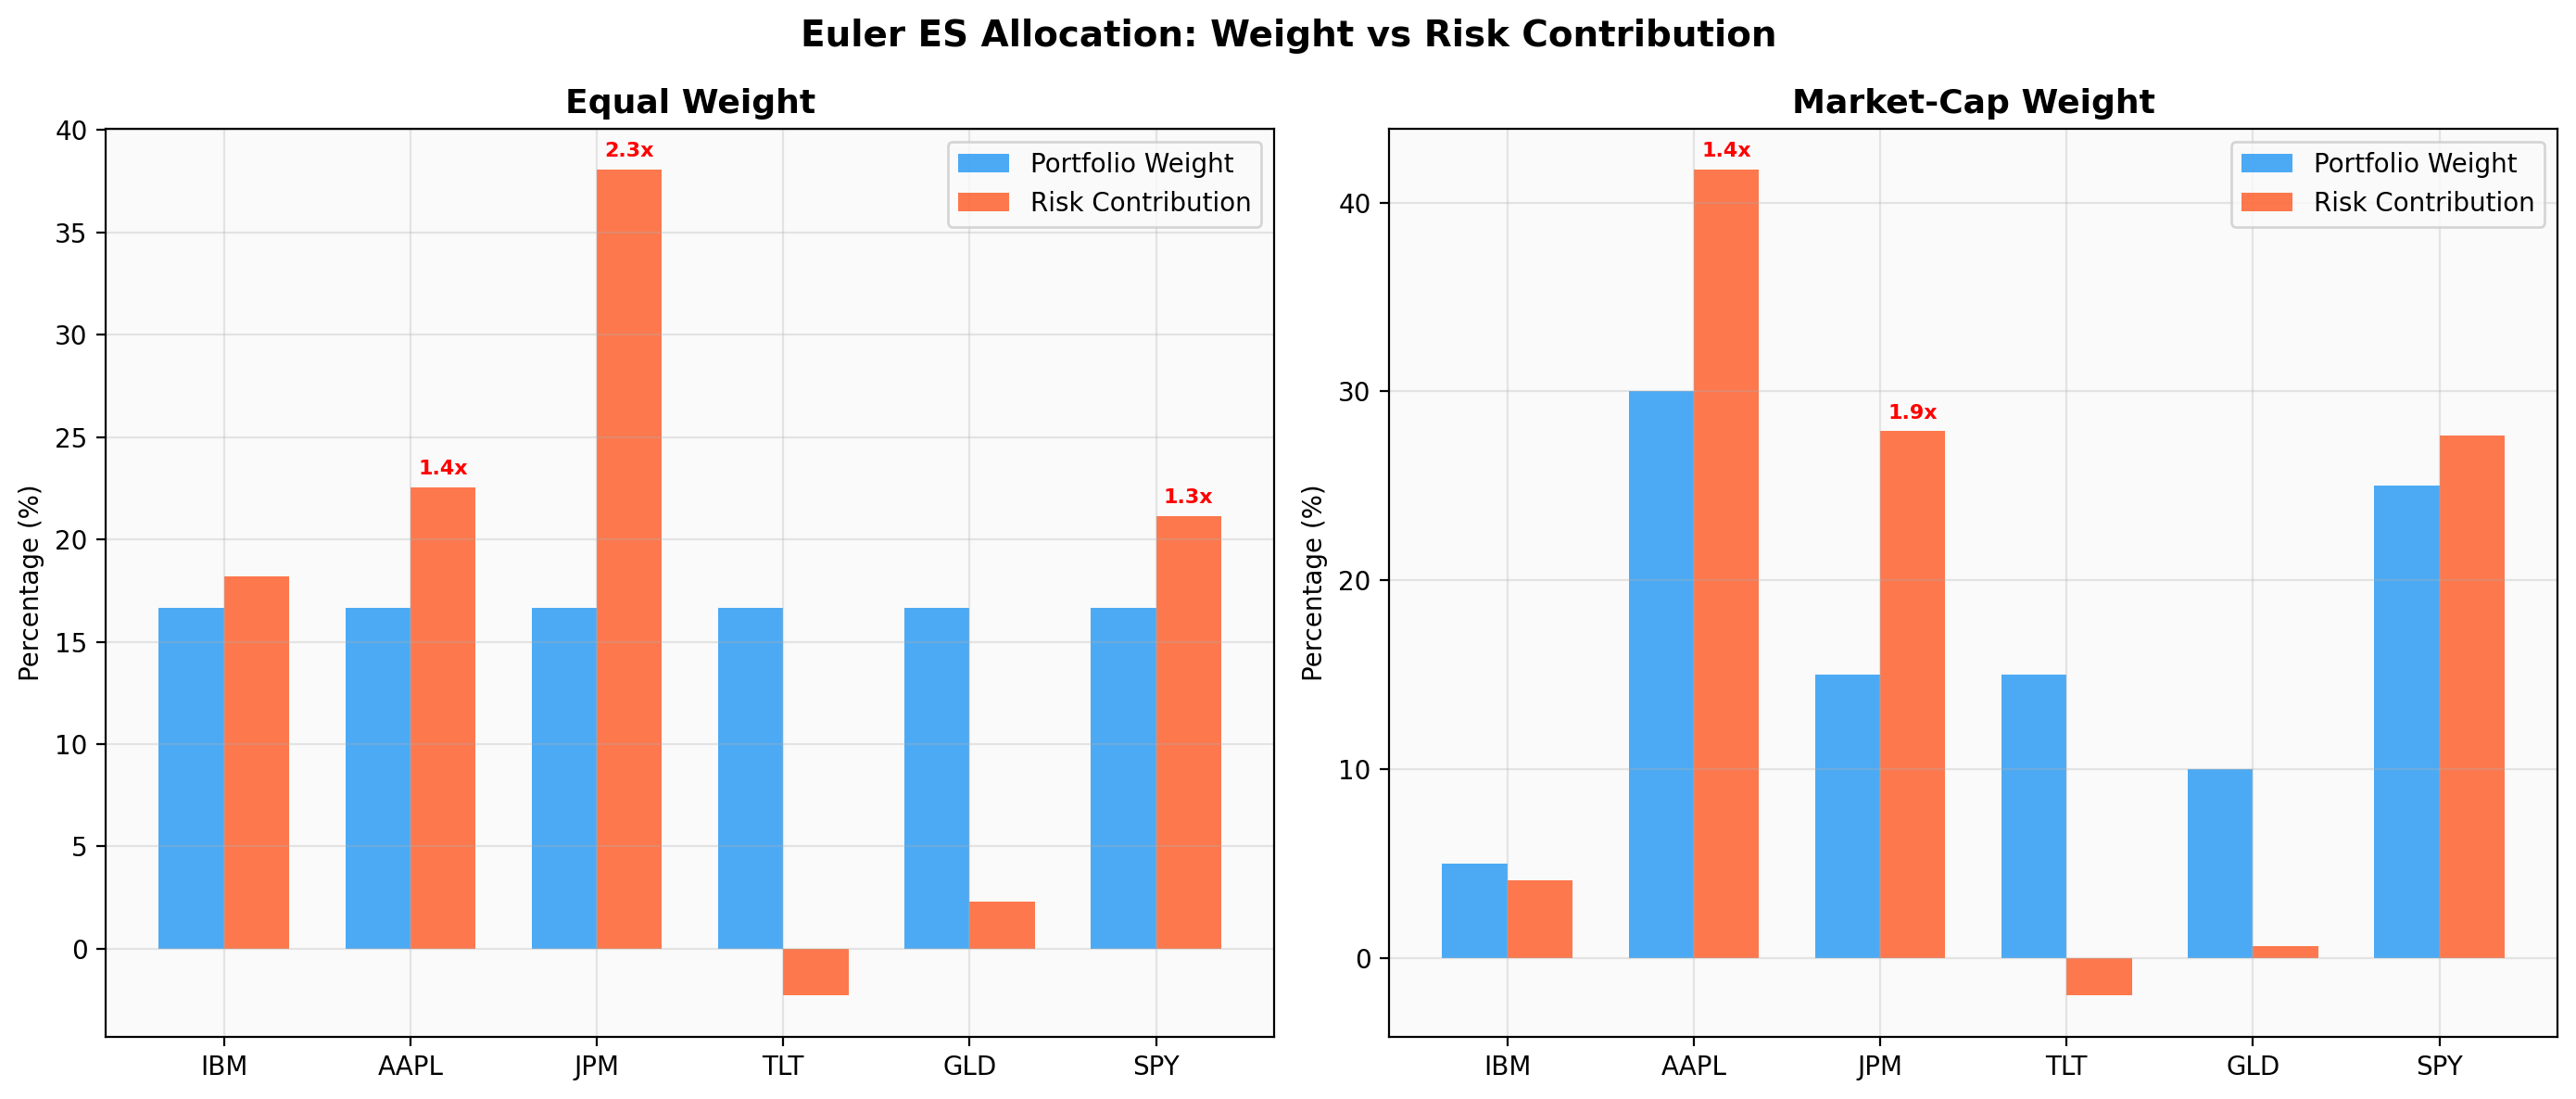
\includegraphics[width=0.85\textwidth]{figures/euler_allocation.png}
    \caption{Euler decomposition of vine copula ES$_{99}$. JPM dominates tail risk (38.1\%) despite holding only 16.7\% weight, while TLT acts as a genuine crash hedge with negative risk contribution ($-$2.3\%).}
    \label{fig:euler}
\end{figure}

\textbf{Regime dependence} analysis confirms that the vine copula captures the crisis correlation increase.
Table~\ref{tab:regime_copula} presents tail dependence coefficients estimated separately on calm and crisis subsamples.

\begin{table}[H]
\centering
\caption{Tail dependence by market regime (selected edges). During crises, tail dependence for equity pairs increases by up to 49$\times$ relative to calm periods, confirming that diversification fails precisely when it is needed most.}
\label{tab:regime_copula}
\small
\begin{tabular}{@{}llrr@{}}
\toprule
\textbf{Edge} & \textbf{Calm $\lambda$} & \textbf{Crisis $\lambda$} & \textbf{Increase} \\
\midrule
Edge 1 & 0.015 & 0.494 & 33$\times$ \\
Edge 2 & 0.007 & 0.494 & 73$\times$ \\
Edge 3 & 0.344 & 0.516 & 1.5$\times$ \\
\bottomrule
\end{tabular}
\end{table}


% ============================================================
\section{Computational Framework}
\label{sec:engine}
% ============================================================

% --- 6.1 Architecture ---
\subsection{C++ Engine Architecture}
\label{sec:cpp}

The simulation engine is implemented in C++20 with OpenMP parallelization.
Three design decisions are critical for performance:

\textbf{CRTP (Curiously Recurring Template Pattern)} enables compile-time polymorphism.
The compiler generates specialized simulation code for each model, inlining the drift and diffusion functions directly into the inner loop.
This eliminates virtual dispatch overhead---significant because the inner loop executes $N_{\text{paths}} \times N_{\text{steps}}$ times (e.g., $100{,}000 \times 252 = 25.2$ million iterations per simulation).

\textbf{Structure-of-Arrays (SoA)} memory layout stores each field (price, variance, auxiliary factors) in contiguous arrays rather than interleaving them per path.
This ensures that the inner loop streams sequentially through memory, maximizing L1/L2 cache utilization and enabling SIMD auto-vectorization.

\textbf{OpenMP thread-level parallelism} distributes paths across CPU cores.
Path-level parallelism is embarrassingly parallel (no inter-path communication), achieving near-linear scaling.
Throughput: GBM at 668K paths/sec, Heston at 500K paths/sec, Rough Heston at 309K paths/sec on 8 threads.

% --- 6.2 Variance Reduction ---
\subsection{Variance Reduction}
\label{sec:vr}

Monte Carlo convergence rate is $O(N^{-1/2})$---halving the standard error requires quadrupling the sample size.
We implement four variance reduction techniques:

\textbf{Sobol quasi-random sequences} \citep{joe2008} replace pseudorandom draws with low-discrepancy sequences that fill the sample space more uniformly.
For mean estimation, Sobol QMC achieves 191$\times$ lower standard error than pseudorandom Monte Carlo at equal sample sizes---effectively replacing $O(N^{-1/2})$ convergence with near-$O(N^{-1})$ convergence.

\textbf{Antithetic variates} exploit the symmetry of the Brownian motion distribution.
For each set of random draws $\{Z_i\}$, we simultaneously simulate with $\{-Z_i\}$.
The two paths are negatively correlated, reducing the variance of the average.
We observe 80\% standard error reduction for ES estimation.

\textbf{Control variates} exploit the analytical tractability of GBM.
Since GBM has known analytical moments, we use the difference between simulated and analytical GBM statistics to correct Heston estimates:
\begin{equation}
\label{eq:cv}
\hat{\mu}_{\text{CV}} = \hat{\mu}_{\text{Heston}} - \beta\bigl(\hat{\mu}_{\text{GBM,sim}} - \mu_{\text{GBM,exact}}\bigr)
\end{equation}
where $\beta$ is the optimal control coefficient.
With a correlation of $\rho = 0.69$ between GBM and Heston terminal values, this achieves 28\% standard error reduction.

\textbf{Importance sampling} tilts the sampling distribution toward the tail region of interest (e.g., the 1\% tail for ES$_{99}$), reducing the variance of tail risk estimates at the cost of slightly higher variance for central statistics.

\begin{figure}[H]
    \centering
    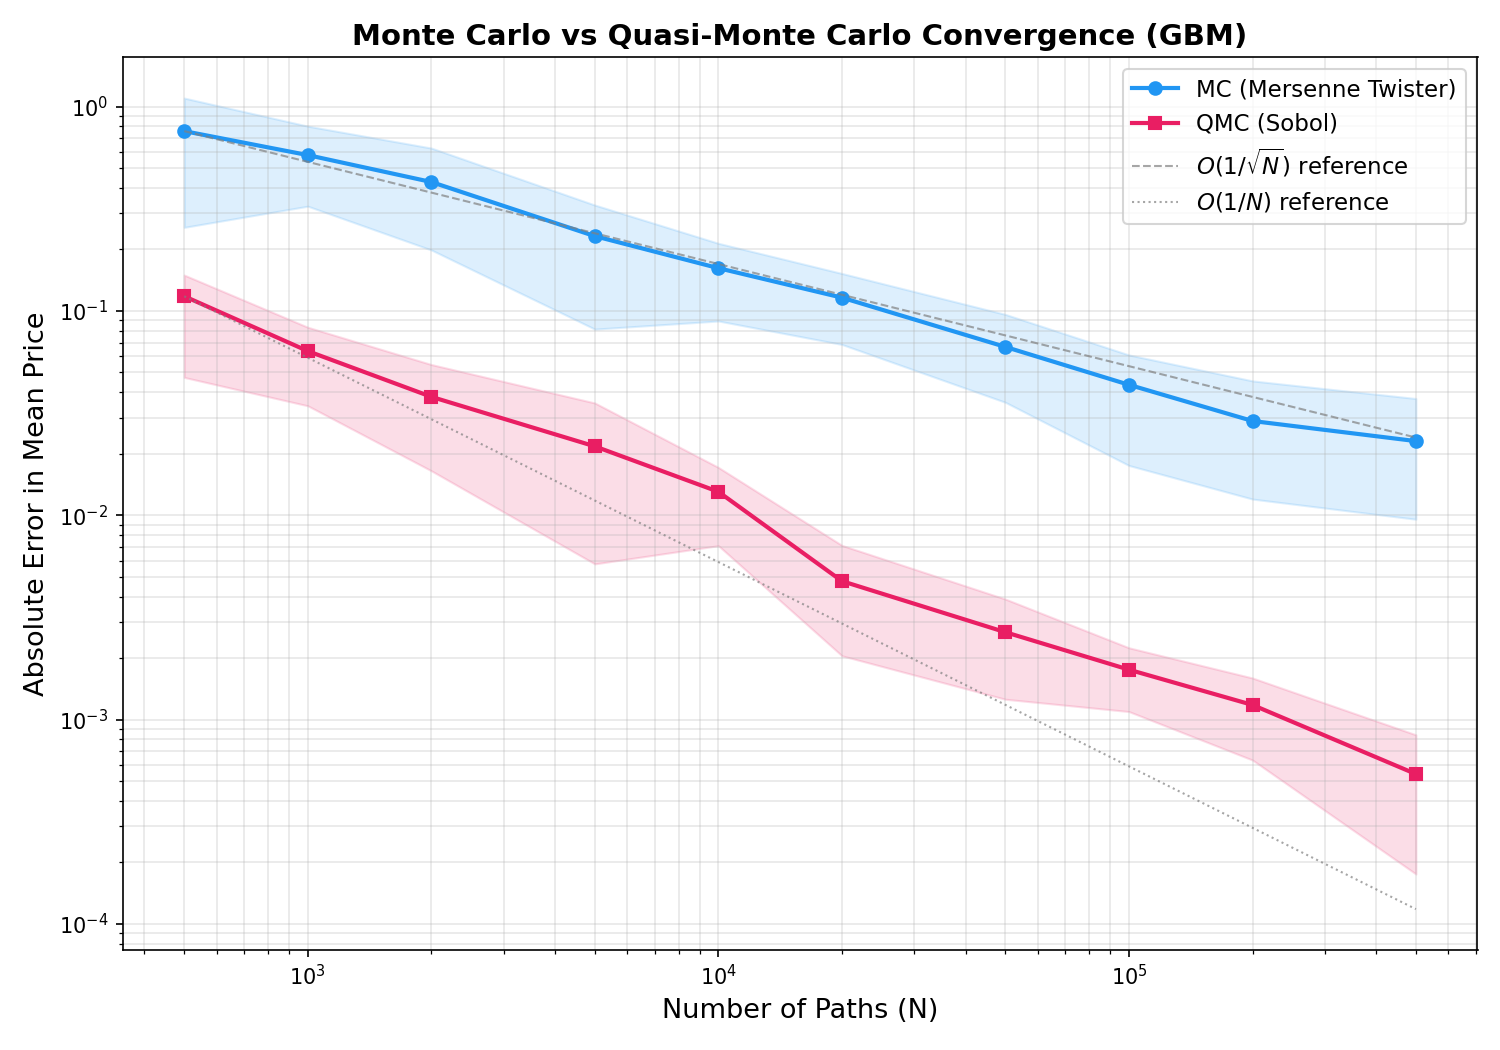
\includegraphics[width=0.95\textwidth]{figures/convergence_comparison.png}
    \caption{Convergence of VaR$_{99}$ estimates as a function of sample size, comparing pseudorandom Monte Carlo (MC), Sobol quasi-Monte Carlo (QMC), and QMC with antithetic variates (QMC+AV). Sobol QMC converges orders of magnitude faster, achieving at 1{,}000 paths the same precision that pseudorandom MC requires 100{,}000+ paths to match.}
    \label{fig:convergence}
\end{figure}

% --- 6.3 Validation ---
\subsection{Validation}
\label{sec:validation}

The C++ engine is validated through 42 unit and integration tests:
\begin{itemize}[leftmargin=1.5em]
    \item \textbf{GBM analytical validation:} Simulated terminal price moments (mean, variance, skewness, kurtosis) are compared against closed-form expressions from Eq.~\eqref{eq:gbm_solution}. All moments match to within 1\% relative error at $10^5$ paths.
    \item \textbf{Heston QE scheme validation:} The QE discretization is tested against the moment-matching conditions of \citet{andersen2008}. Variance paths remain non-negative in all simulations ($10^6$ paths), and the distribution of terminal variance matches the known non-central $\chi^2$ distribution.
    \item \textbf{Rough Heston kernel validation:} At $H = 0.5$, Rough Heston output is verified to match classical Heston output to within Monte Carlo noise, confirming correct kernel implementation.
    \item \textbf{Calibration fit:} Simulated return moments (variance, skewness, kurtosis) under calibrated parameters are compared against empirical values. For SPY under Heston: simulated variance 0.0366 vs.\ empirical 0.0371 (1.3\% error); simulated kurtosis 16.16 vs.\ empirical 15.88 (1.7\% error).
\end{itemize}


% ============================================================
\section{Empirical Results}
\label{sec:results}
% ============================================================

% --- 7.1 Three-Model Risk Comparison ---
\subsection{Three-Model Risk Comparison}
\label{sec:risk_comparison}

Table~\ref{tab:three_model} presents risk metrics from 100{,}000-path simulations under each volatility model, using parameters calibrated to SPY historical returns.
All metrics are expressed per \$100 notional investment.

\begin{table}[H]
\centering
\caption{Risk metrics across the three volatility models (SPY, 100{,}000 paths, 1-year horizon). The ``Model Risk'' column shows the percentage difference between the most and least conservative estimate. The 31\% spread in ES$_{99}$ arises purely from model choice applied to identical data.}
\label{tab:three_model}
\small
\begin{tabular}{@{}lrrrr@{}}
\toprule
\textbf{Metric} & \textbf{GBM} & \textbf{Heston} & \textbf{Rough Heston} & \textbf{Model Risk} \\
\midrule
VaR$_{95}$ (\$) & 22.83 & 28.52 & 28.65 & 25\% \\
VaR$_{99}$ (\$) & 35.36 & 44.58 & 44.78 & 27\% \\
ES$_{95}$ (\$)  & 28.77 & 36.72 & 36.95 & 28\% \\
ES$_{99}$ (\$)  & 39.52 & 51.31 & 51.81 & 31\% \\
Skewness         & +0.61  & $-$0.22 & $-$0.22 & sign reversal \\
Ex.\ Kurtosis    & 0.67  & 0.02   & 0.04   & --- \\
\bottomrule
\end{tabular}
\end{table}

A risk manager using GBM estimates ES$_{99}$ of \$39.52 per \$100 invested.
Under Heston, the same metric is \$51.31---a 30\% increase.
This gap is \emph{pure model risk}: it arises not from different market data or different time periods, but solely from the choice of mathematical framework applied to identical inputs.
To put this in perspective: a fund managing \$1 billion with GBM-based risk estimates would hold \$395M in reserves for tail losses; Heston would suggest \$513M---a difference of \$118M in capital adequacy.

The skewness difference is equally telling.
GBM produces \emph{positive} skewness (+0.61) due to the log-normal distribution's right skew---implying that large upward moves are more likely than large downward moves.
Heston produces \emph{negative} skewness ($-$0.22), matching the empirical observation that equity markets crash more violently than they rally.
A risk system based on GBM not only underestimates the magnitude of tail losses but mischaracterizes their direction.

% --- 7.2 Walk-Forward Backtesting ---
\subsection{Walk-Forward Backtesting}
\label{sec:backtest}

We evaluate all models through walk-forward backtesting on 1{,}053 trading days (2022--2025).
Each day, parameters are recalibrated on the expanding historical window, 10{,}000 paths are simulated, and the 1\% VaR is computed.
An \emph{exceedance} occurs when the realized loss exceeds the predicted VaR.

\textbf{Kupiec unconditional coverage test} \citep{kupiec1995}.
Under the null hypothesis that the model is correctly specified, the expected number of exceedances in $T = 1{,}053$ days at the $\alpha = 1\%$ level is $T \cdot \alpha = 10.53$.
The Kupiec likelihood ratio test statistic is:
\begin{equation}
\label{eq:kupiec}
LR_{\text{uc}} = -2\ln\!\left[\frac{\alpha^x (1-\alpha)^{T-x}}{\hat{\pi}^x (1-\hat{\pi})^{T-x}}\right]
\end{equation}
where $x$ is the observed number of exceedances and $\hat{\pi} = x/T$ is the empirical exceedance rate.
Under $H_0$, $LR_{\text{uc}} \sim \chi^2(1)$.

\textbf{Christoffersen conditional coverage test} \citep{christoffersen1998}.
Tests both correct coverage \emph{and} independence of exceedances.
The independence component tests whether the probability of an exceedance depends on whether the previous day was also an exceedance.

Table~\ref{tab:backtest} presents the results.

\begin{table}[H]
\centering
\caption{Walk-forward backtesting results (VaR$_{99}$, 1{,}053 test days, SPY). Expected exceedances: 10.53. Kupiec tests unconditional coverage; Christoffersen tests conditional coverage (coverage + independence). Basel traffic light zones are evaluated on the most recent 250 trading days per the standard regulatory convention: green ($\leq 4$), yellow (5--9), red ($\geq 10$).}
\label{tab:backtest}
\small
\begin{tabular}{@{}lrrrrrl@{}}
\toprule
\textbf{Model} & \textbf{Exc.} & \textbf{Rate} & \textbf{Kupiec $p$} & \textbf{Christ.\ $p$} & \textbf{Cluster} & \textbf{Basel} \\
\midrule
ARIMA         & 15 & 1.42\% & 0.193          & \textbf{0.023} & 10.64$\times$ & Green  \\
GBM           & 22 & 2.09\% & \textbf{0.002} & \textbf{0.002} & 5.60$\times$  & Yellow \\
Heston        & 14 & 1.33\% & 0.306          & 0.237          & 5.70$\times$  & Green  \\
Rough Heston  & 14 & 1.33\% & 0.306          & 0.237          & 5.70$\times$  & Green  \\
\bottomrule
\end{tabular}
\end{table}

\textbf{GBM is formally rejected} by the Kupiec test ($p = 0.002$), producing 22 exceedances against an expected 10.53.
Beyond the statistical rejection, the practical consequence is significant: during our test period, a GBM-based risk system would have triggered 22 days where actual losses exceeded the stated worst case---an event that should occur only 10--11 times if the model were correct.
Each such exceedance represents a day where the institution's actual exposure exceeded its perceived exposure.

\textbf{ARIMA presents a subtler failure.}
With 15 exceedances, it passes the Kupiec test ($p = 0.193$)---its average exceedance rate is close to the target.
However, the Christoffersen independence test rejects ($p = 0.023$), with a clustering ratio of 10.64$\times$.
If ARIMA's VaR was violated today, it is 10.64 times more likely to be violated again tomorrow than on a random day.
This clustering means that ARIMA's failures concentrate into multi-day streaks---precisely the scenario that produces the largest cumulative losses.

\textbf{Heston and Rough Heston both pass} at all significance levels, achieving Basel Green status with 14 exceedances each.
Their clustering ratios (5.70$\times$) are lower than ARIMA's, indicating better-calibrated uncertainty estimates.

\begin{figure}[H]
    \centering
    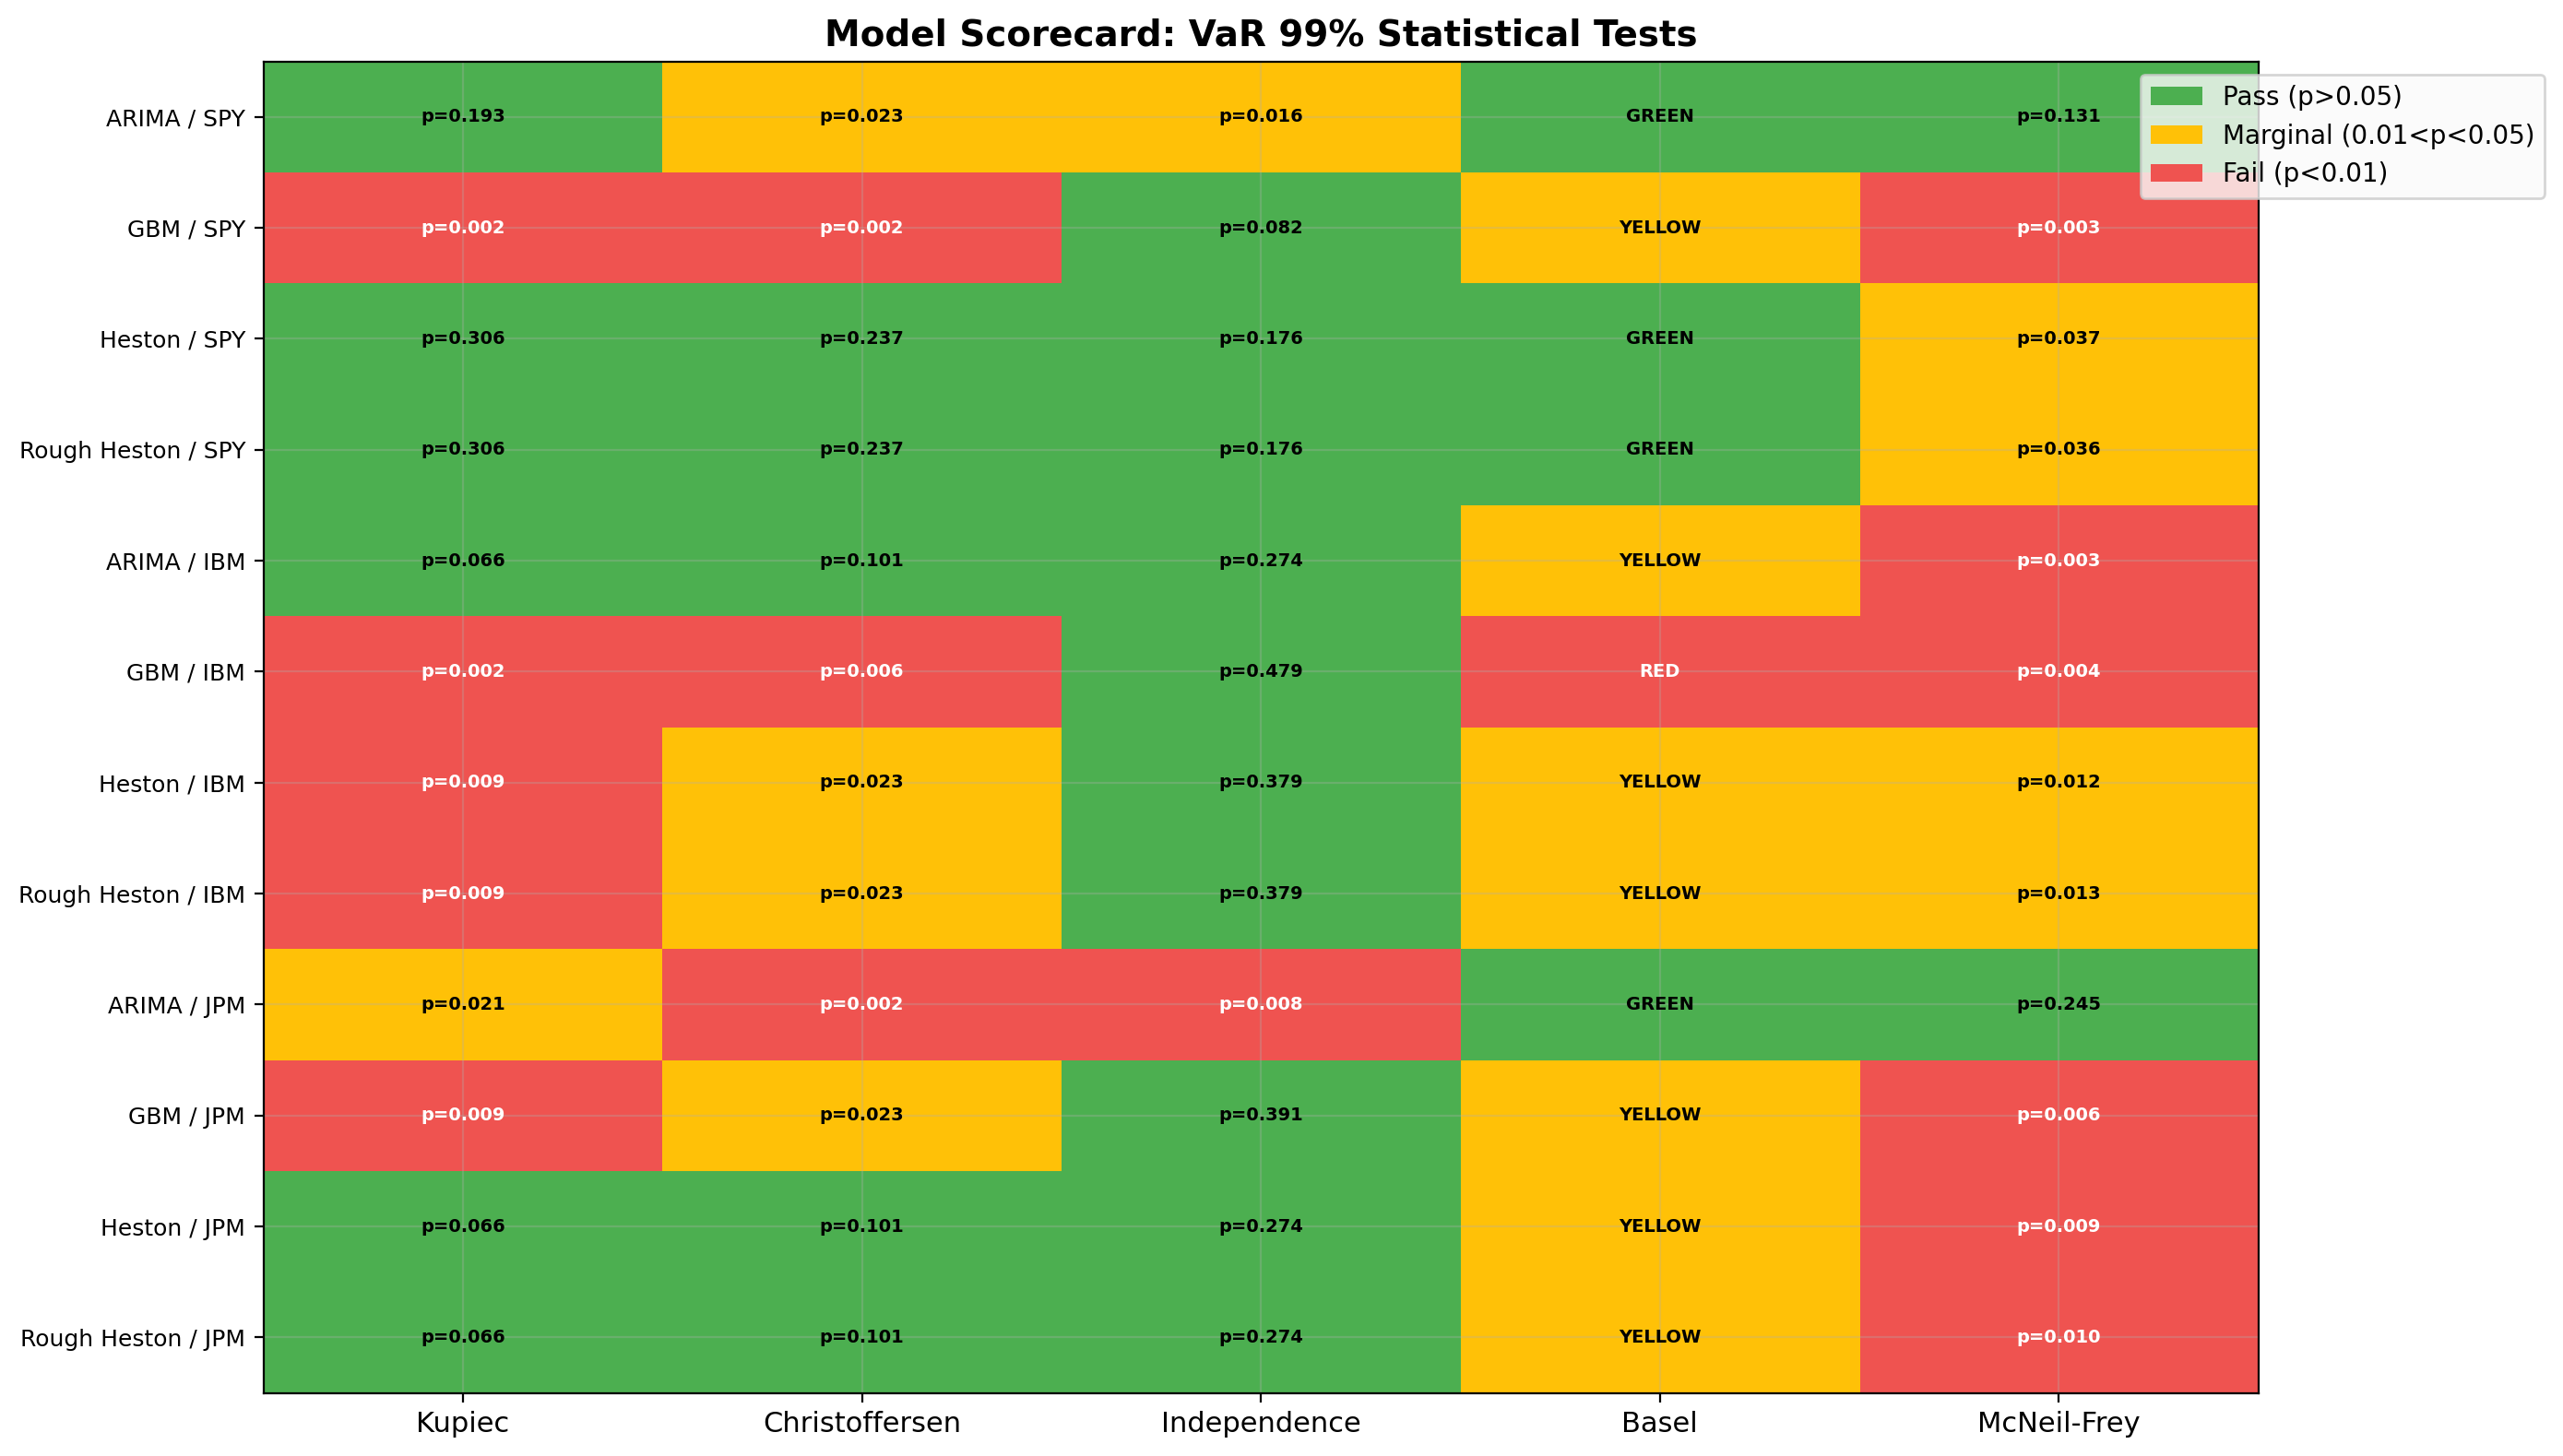
\includegraphics[width=\textwidth]{figures/model_scorecard.png}
    \caption{Model scorecard heatmap summarizing backtesting results across models, assets, and test criteria. Green cells indicate the test is passed; red cells indicate rejection at the 5\% significance level. Heston and Rough Heston achieve the most green cells across all criteria.}
    \label{fig:scorecard}
\end{figure}

% --- 7.3 Regime Analysis ---
\subsection{Regime Analysis}
\label{sec:regime}

Table~\ref{tab:regime} disaggregates backtesting results by market regime.

\begin{table}[H]
\centering
\caption{VaR$_{99}$ exceedance rates by regime (SPY, 1{,}053 test days: 892 calm, 161 crisis). The target rate is 1\%. GBM's crisis exceedance rate of 12.42\% is 12$\times$ the target; Heston's 6.21\% is still elevated but substantially better calibrated.}
\label{tab:regime}
\small
\begin{tabular}{@{}lrrrr@{}}
\toprule
\textbf{Model} & \textbf{Calm Exc.} & \textbf{Calm Rate} & \textbf{Crisis Exc.} & \textbf{Crisis Rate} \\
\midrule
ARIMA        & 0  & 0.00\%  & 15 & 9.32\%  \\
GBM          & 2  & 0.22\%  & 20 & 12.42\% \\
Heston       & 4  & 0.45\%  & 10 & 6.21\%  \\
Rough Heston & 4  & 0.45\%  & 10 & 6.21\%  \\
\bottomrule
\end{tabular}
\end{table}

The regime decomposition reveals the mechanism behind each model's failure mode:

\textbf{ARIMA:} Zero exceedances during calm periods, all 15 concentrated in crises (9.32\% rate).
This is a direct consequence of constant-width prediction intervals: during calm periods, the intervals are too wide (wasting capital with a 0\% exceedance rate versus the 1\% target); during crises, they are too narrow.
ARIMA achieves acceptable \emph{average} coverage by exactly offsetting its calm-period conservatism with crisis-period failure.

\textbf{GBM:} 12.42\% crisis exceedance rate means that on approximately one in eight crisis days, losses exceed the stated VaR---twelve times the target rate.
GBM's constant-volatility assumption ensures that its risk estimates cannot adapt to heightened market stress.

\textbf{Heston:} 6.21\% crisis exceedance rate---still elevated above the 1\% target, but substantially better than GBM.
Heston's stochastic volatility process allows risk estimates to increase during volatile periods, though the calibration lag means it responds with some delay to sudden regime changes.

% --- 7.4 Dynamic Hedging ---
\subsection{Dynamic Hedging: The Dollar Cost of Model Risk}
\label{sec:hedging}

To translate statistical model differences into financial terms, we simulate a delta hedging strategy for a 3-month at-the-money European call option on SPY with \$10M notional.

A trader who prices and hedges under GBM (Black--Scholes delta) but operates in a world governed by stochastic volatility will experience larger and more skewed hedge losses than expected.
Table~\ref{tab:hedging} presents the results.

\begin{table}[H]
\centering
\caption{Hedge P\&L statistics per \$100 notional (10{,}000 simulated hedging episodes). ``GBM true'' is the baseline where the world is actually GBM and the trader uses BS delta. ``Heston true'' and ``Rough Heston true'' simulate worlds where the actual dynamics follow stochastic volatility but the trader uses constant-volatility BS delta. The ``constant'' strategy uses Black--Scholes delta; ``local vol'' uses the Heston-aware delta.}
\label{tab:hedging}
\small
\begin{tabular}{@{}llrrrr@{}}
\toprule
\textbf{True Model} & \textbf{Strategy} & \textbf{Mean P\&L} & \textbf{Std} & \textbf{VaR$_{99}$} & \textbf{ES$_{99}$} \\
\midrule
GBM          & BS delta    & \$0.66  & \$0.52  & \$0.62  & \$0.90  \\
Heston       & BS delta    & \$2.24  & \$1.72  & \$3.62  & \$5.53  \\
Heston       & local vol   & \$2.35  & \$1.74  & \$3.08  & \$4.15  \\
Rough Heston & BS delta    & \$1.09  & \$2.34  & \$7.42  & \$10.42 \\
\bottomrule
\end{tabular}
\end{table}

On a \$10M notional SPY position, a Black--Scholes-assuming trader who sells a 3-month call and delta-hedges daily expects a worst-case (99th percentile) hedge loss of \$90{,}000 (ES$_{99}$, scaled from per-\$100 figures).
Under Heston-calibrated dynamics, the true 99th-percentile loss is \$553{,}000; under Rough Heston, it is \$1{,}042{,}000.
This is hidden risk: the trader's reserves are insufficient by a factor of 6 to 12$\times$, with the shortfall materializing precisely during the volatile periods that produce the largest option movements.

The kurtosis of hedge P\&L increases dramatically: from 0.15 under GBM to 6.11 under Heston and 9.03 under Rough Heston.
This means that not only are extreme losses larger, they are \emph{far more frequent} relative to the average loss than the trader's model predicts.

The ``local vol'' hedging strategy---which uses the Heston-aware delta rather than the constant-volatility BS delta---reduces ES$_{99}$ from \$5.53 to \$4.15 (25\% reduction).
While this demonstrates that model-aware hedging partially mitigates model risk, the residual risk (\$4.15 vs.\ baseline \$0.90) confirms that stochastic volatility introduces irreducible hedging uncertainty that cannot be eliminated by delta hedging alone.

\begin{figure}[H]
    \centering
    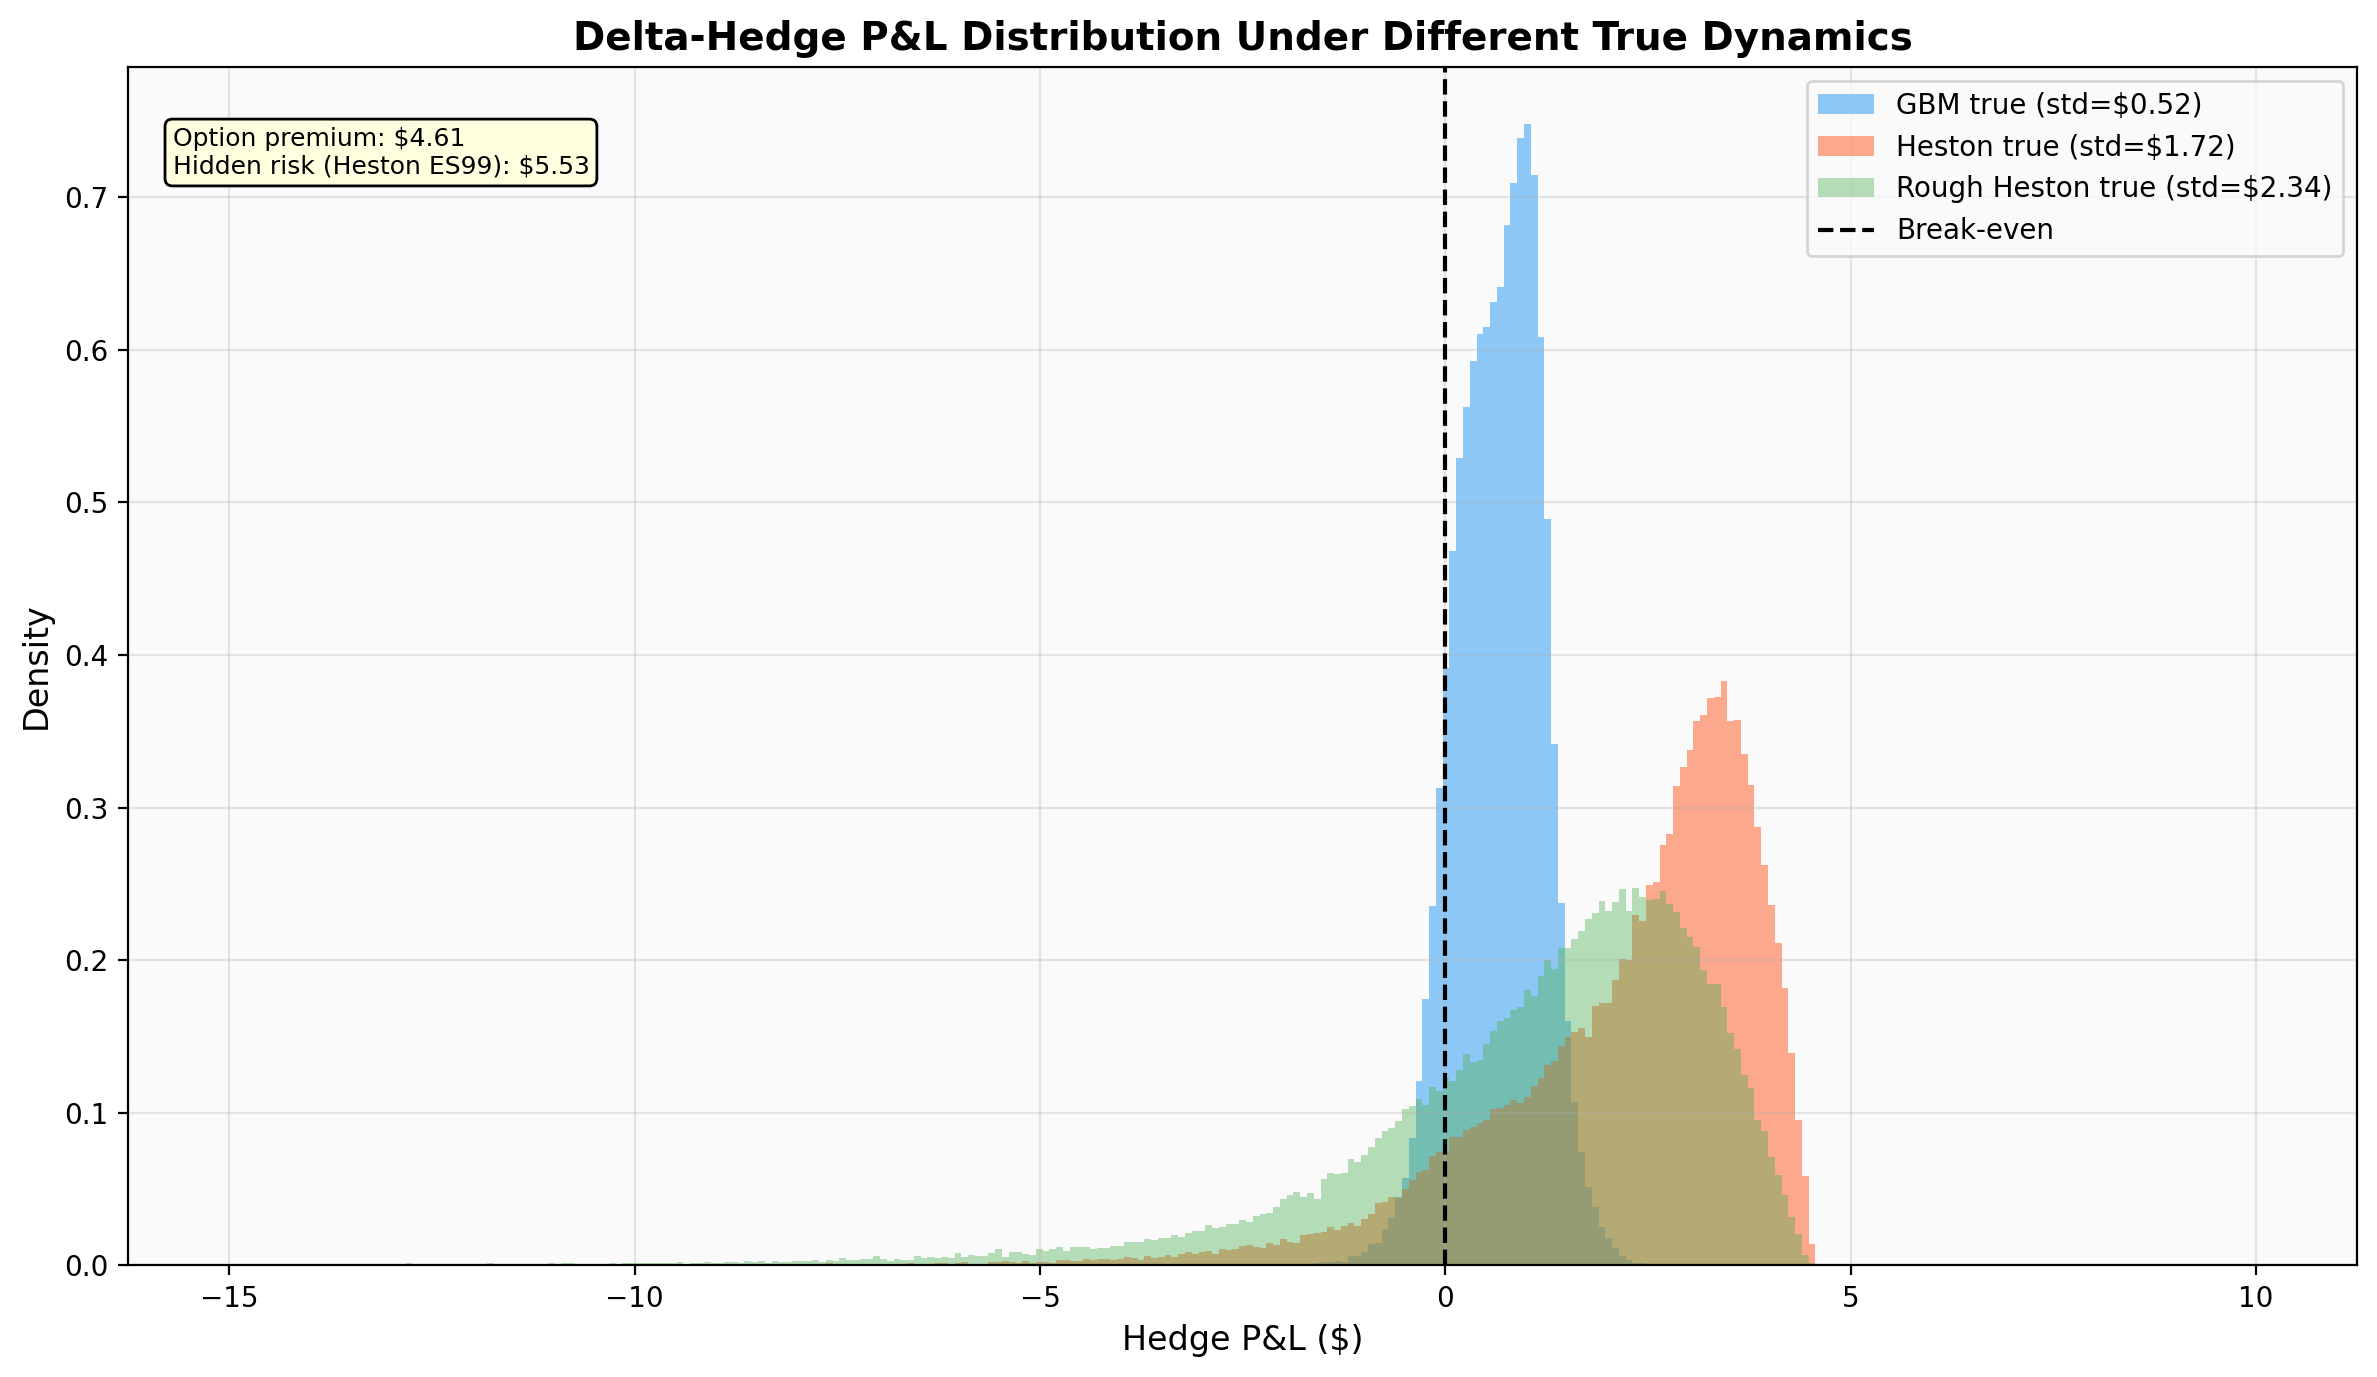
\includegraphics[width=\textwidth]{figures/hedge_pnl_distributions.png}
    \caption{Hedge P\&L distributions under the three true-world models. The GBM baseline (blue) is tightly concentrated. Heston (orange) and Rough Heston (green) exhibit dramatically heavier left tails---the hidden risk that a Black--Scholes-assuming trader does not account for.}
    \label{fig:hedge_pnl}
\end{figure}


% ============================================================
\section{Discussion and Limitations}
\label{sec:discussion}
% ============================================================

We acknowledge several limitations of this study that should inform the interpretation of our results:

\textbf{1.\ Calibration methodology.}
Our parameters are calibrated via maximum likelihood estimation on historical returns.
This approach reproduces historical return distributions but may not match current market pricing of options.
Calibration to implied volatility surfaces---the standard in derivatives practice---would produce parameters that reflect market expectations rather than historical realizations.
The two approaches can yield substantially different parameter estimates, particularly for $\rho$ and $\sigma_v$.

\textbf{2.\ Backtest horizon.}
The walk-forward backtest covers 1{,}053 days (approximately 4 years, 2022--2025).
While this period includes meaningful volatility regimes (2022 inflation shock, 2023 banking crisis, 2024--2025 recovery), it does not span a full market cycle or a systemic event comparable to 2008.
A longer test period spanning multiple complete cycles would strengthen the conclusions, particularly for the Rough Heston model where the long-memory property is most relevant on multi-year horizons.

\textbf{3.\ Heston vs.\ Rough Heston similarity.}
On our 1-day VaR backtest, Heston and Rough Heston produce nearly identical results (14 exceedances each, identical $p$-values).
The differentiation between these models would be more pronounced on longer horizons (weekly or monthly VaR), on option pricing tasks where the term structure of implied volatility matters, or in the ATM skew dynamics where roughness has the most impact.

\textbf{4.\ Static copula.}
The vine copula is estimated on the full training set and held constant during the test period.
A dynamic copula that adapts to regime changes---for example, through a regime-switching or DCC (Dynamic Conditional Correlation) approach \citep{engle1982}---would better capture the time-varying nature of dependence documented in Table~\ref{tab:regime_copula}.

\textbf{5.\ Transaction costs.}
The hedging simulation ignores transaction costs.
In practice, the higher-frequency rebalancing required by stochastic volatility models incurs additional trading costs that partially offset the improved hedge quality.
The net benefit of model-aware hedging after transaction costs is an important question for future work.

\textbf{6.\ Parameter uncertainty.}
We report risk metrics conditional on point-estimated parameters.
In reality, parameters are estimated with uncertainty, and this parameter uncertainty propagates into risk estimates.
A Bayesian approach that marginalizes over parameter posterior distributions would provide more honest uncertainty quantification, at the cost of substantially increased computational burden.


% ============================================================
\section{Conclusions}
\label{sec:conclusion}
% ============================================================

This paper has constructed and validated a computational framework for quantifying model risk in multi-asset portfolios.
Three principal findings emerge:

\textbf{1.\ Model risk is quantifiable and material.}
Expected Shortfall at the 99\% level diverges by 31\% across the GBM--Heston--Rough Heston hierarchy (Table~\ref{tab:three_model}), and vine copula dependence adds a further 15\% to tail risk relative to the Gaussian copula (Table~\ref{tab:copula_risk}).
The combined effect exceeds 40\%: a risk system using GBM with Gaussian dependence underestimates portfolio tail risk by more than 40\% relative to one using Heston with vine copula dependence.
This gap is comparable in magnitude to the market risk itself, yet is entirely invisible to a practitioner using a single model.

\textbf{2.\ Stochastic volatility produces calibrated prediction intervals where deterministic models fail.}
In formal walk-forward backtesting on 1{,}053 days of real market data, GBM is rejected by the Kupiec test ($p = 0.002$) and ARIMA fails the Christoffersen independence test ($p = 0.023$) with a clustering ratio of 10.64$\times$.
Heston and Rough Heston pass both tests, achieving Basel Green status (Table~\ref{tab:backtest}).
The regime analysis reveals the mechanism: GBM's crisis exceedance rate is 12.42\% versus a 1\% target, while Heston achieves 6.21\% (Table~\ref{tab:regime}).

\textbf{3.\ Model risk translates to concrete dollar amounts in hedging.}
On a \$10M notional equity position, a Black--Scholes-assuming delta hedger underestimates 99th-percentile hedge losses by \$460{,}000 to \$950{,}000 depending on whether the true dynamics follow Heston or Rough Heston (Table~\ref{tab:hedging}).
This ``hidden risk'' compounds during volatile periods and is not captured by any analysis based on the constant-volatility assumption.

The overarching conclusion is that \textbf{model risk is not an abstract regulatory concern but a concrete, quantifiable financial exposure}.
The magnitude of this exposure---30\% on ES, 6--12$\times$ on hedge tail risk---should inform both regulatory capital requirements and institutional risk management practice.
Rather than committing to a single ``best'' model, risk-aware practitioners should maintain a hierarchy of models and report the \emph{range} of risk estimates as a measure of model uncertainty.
The computational framework presented here, combining high-performance C++ simulation with rigorous statistical backtesting, provides a practical platform for doing so.


% ============================================================
% REFERENCES
% ============================================================
\bibliographystyle{apalike}
\bibliography{references}

\end{document}
